%%%%%%%%%%%%%%%%%%%%%%%%%%%%%%%%%%%%%%%%%
% Journal Article
% LaTeX Template
% Version 1.4 (15/5/16)
%
% This template has been downloaded from:
% http://www.LaTeXTemplates.com
%
% Original author:
% Frits Wenneker (http://www.howtotex.com) with extensive modifications by
% Vel (vel@LaTeXTemplates.com)
%
% License:
% CC BY-NC-SA 3.0 (http://creativecommons.org/licenses/by-nc-sa/3.0/)
%
%%%%%%%%%%%%%%%%%%%%%%%%%%%%%%%%%%%%%%%%%

%----------------------------------------------------------------------------------------
%	PACKAGES AND OTHER DOCUMENT CONFIGURATIONS
%----------------------------------------------------------------------------------------

%\documentclass{article}
\documentclass[oneside,twocolumn]{article}

\usepackage{blindtext} % Package to generate dummy text throughout this template 
\usepackage{multicol}
\usepackage[sc]{mathpazo} % Use the Palatino font
\usepackage[T1]{fontenc} % Use 8-bit encoding that has 256 glyphs
\linespread{1.05} % Line spacing - Palatino needs more space between lines
\usepackage{microtype} % Slightly tweak font spacing for aesthetics

%\usepackage[english]{babel} % Language hyphenation and typographical rules
\usepackage[spanish]{babel}
\usepackage[hmarginratio=1:1,top=32mm,columnsep=20pt]{geometry} % Document margins
\usepackage[hang, small,labelfont=bf,up,textfont=it,up]{caption} % Custom captions under/above floats in tables or figures
\usepackage{booktabs} % Horizontal rules in tables

\usepackage{lettrine} % The lettrine is the first enlarged letter at the beginning of the text

\usepackage{listings} % Required for insertion of code

\usepackage{enumitem} % Customized lists
\setlist[itemize]{noitemsep} % Make itemize lists more compact

\usepackage{abstract} % Allows abstract customization
\renewcommand{\abstractnamefont}{\normalfont\bfseries} % Set the "Abstract" text to bold
\renewcommand{\abstracttextfont}{\normalfont\small\itshape} % Set the abstract itself to small italic text

\usepackage{titlesec} % Allows customization of titles
\renewcommand\thesection{\Roman{section}} % Roman numerals for the sections
\renewcommand\thesubsection{\roman{subsection}} % roman numerals for subsections
\titleformat{\section}[block]{\large\scshape\centering}{\thesection.}{1em}{} % Change the look of the section titles
\titleformat{\subsection}[block]{\large}{\thesubsection.}{1em}{} % Change the look of the section titles

\usepackage{fancyhdr} % Headers and footers
\pagestyle{fancy} % All pages have headers and footers
\fancyhead{} % Blank out the default header
\fancyfoot{} % Blank out the default footer
%\fancyhead[C]{Running title $\bullet$ May 2016 $\bullet$ Vol. XXI, No. 1} % Custom header text
\fancyfoot[RO,LE]{\thepage} % Custom footer text

\usepackage{titling} % Customizing the title section

\usepackage{hyperref} % For hyperlinks in the PDF

\usepackage{listings}
\usepackage{algorithm2e}
\usepackage{graphicx}
\usepackage[dvipsnames]{xcolor}
\definecolor{codegreen}{rgb}{0,0.6,0}
\definecolor{codegray}{rgb}{0.5,0.5,0.5}
\definecolor{codepurple}{rgb}{0.58,0,0.82}
\definecolor{backcolour}{rgb}{1,1,1}
\lstdefinestyle{mystyle}{
    backgroundcolor=\color{backcolour},   
    commentstyle=\color{codegreen},
    keywordstyle=\color{magenta},
    numberstyle=\tiny\color{codegray},
    stringstyle=\color{codepurple},
    basicstyle=\ttfamily\footnotesize,
    breakatwhitespace=false,         
    breaklines=true,                 
    captionpos=b,                    
    keepspaces=true,                 
    numbers=left,                    
    numbersep=5pt,                  
    showspaces=false,                
    showstringspaces=false,
    showtabs=false,                  
    tabsize=2
}
\renewcommand{\lstlistingname}{Código}% Listing -> Algorithm
\lstset{style=mystyle}

\usepackage[utf8]{inputenc} % Required for inputting international characters
\usepackage[T1]{fontenc} % Output font encoding for international characters

\usepackage{amsmath}
%----------------------------------------------------------------------------------------
%	TITLE SECTION
%----------------------------------------------------------------------------------------

\setlength{\droptitle}{-4\baselineskip} % Move the title up

\pretitle{\begin{center}\Huge\bfseries} % Article title formatting
\posttitle{\end{center}} % Article title closing formatting
\title{Ley de Control no lineal} % Article title
\author{%
\textsc{Luis Alberto Ballado Aradias} \\%\thanks{A thank you or further information} \\[1ex] % Your name
\normalsize Cinvestav Unidad Tamaulipas \\ % Your institution
\normalsize \href{mailto:luis.ballado@cinvestav.mx}{luis.ballado@cinvestav.mx} % Your email address
%\and % Uncomment if 2 authors are required, duplicate these 4 lines if more
%\textsc{Jane Smith}\thanks{Corresponding author} \\[1ex] % Second author's name
%\normalsize University of Utah \\ % Second author's institution
%\normalsize \href{mailto:jane@smith.com}{jane@smith.com} % Second author's email address
}
\date{\today} % Leave empty to omit a date
\renewcommand{\maketitlehookd}{%
  \begin{abstract}
    \noindent El presente trabajo describe el uso de odometría para un robot móvil de tipo diferencial y su implementación utilizando un robot LEGO NXT bajo el lenguaje NXC (Not eXactly C). La odometría es una técnica utilizada en robótica móvil diferencial para estimar la posición y orientación de un robot mientras se mueve en un entorno. En robots móviles diferenciales, la odometría se basa en la medición de las velocidades de las ruedas y el diámetro de las mismas. La integración de las velocidades permite obtener una estimación de la trayectoria seguida por el robot, pero los errores acumulativos pueden afectar la precisión de la estimación.
  \end{abstract}
}

%----------------------------------------------------------------------------------------

\begin{document}

% Print the title
\maketitle

%----------------------------------------------------------------------------------------
%	ARTICLE CONTENTS
%----------------------------------------------------------------------------------------

\section{Introducción}

\lettrine[nindent=0em,lines=3]{L}a odometría es el estudio de la estimación de la posición de vehículos con ruedas durante la navegación. Para realizar esta estimación se usa información sobre la rotación de las ruedas para estimar cambios en la posición a lo largo del tiempo. El término se usa a veces para referirse a la distancia que ha recorrido uno de estos vehículos.\\

La palabra \textbf{odometría} se compone por las palabras griegas \textbf{hodos} (viajar,trayecto) y \textbf{metron} (medida). La idea fundamental es la integración de información incremental del movimiento a lo largo del tiempo.\\

A pesar de las limitaciones, es una parte importante del sistema de navegación de un robot debido a su bajo costo y esfuerzo de implementación, debe usarse con medidas del posicionamiento absolutas para proporcionar una estimación de la posición más fiable.\\

Hay casos, cuando no hay referencias externas, la odometría es la única información de navegación utilizando un modelo matemático que tiene en cuenta las catacterísticas del movimiento del robot y la geometría del entorno. %Este modelo permite predecir la posición y orientación del robot a medida que se mueve, lo que puede ser utilizado para planificar trayectorias.\\

%La odometría es una técnica fundamental en la navegación autónoma de robots móviles, ya que permite que el robot tenga una estimación en tiempo real de su posición en el entorno y, y por lo tanto, pueda tomar decisiones en función de esta información.

\subsection{Pasos de la odometría}

La metodología para realizar odometría en robots móviles depende del tipo de robot y de los sensores utilizados, pero en general, se pueden seguir los siguientes pasos:
\begin{enumerate}
\item Caracterización de las ruedas: se debe medir el radio de las ruedas y distancia entre el punto de contacto entre cada rueda.
\item Adquisición de datos: se deben medir las velocidades de las ruedas y la dirección de giro del robot. Esto se puede realizar mediante encoders en las ruedas o mediante sensores inerciales.
\item Integración de las velocidades: se deben integrar las velocidades medidas para calcular la posición y orientación del robot.
\item Corrección de errores: se deben corregir los errores que pueden afectar la precisión de la odometría, como el deslizamiento de las ruedas, la fricción con el suelo o la deformación de los neumáticos.
\item Evaluación de la precisión: se deben evaluar la precisión y el error de la odometría. Para ellos, se pueden comparar las estimaciones obtenidas con la posición real del robot o con la información obtenida por otros sensores.
\end{enumerate}

%------------------------------------------------

\newpage
\onecolumn
\section{Métodos}

\subsection{Instalación}

Comenzaremos con la instalación de NXC (Not Exactly C)\\

La configuración del compilador se realiza para un ambiente \textbf{LINUX Ubuntu 20.04LTS}

\begin{enumerate}
\item Verificar si podemos reconocer el bloque NXT con el siguiente comando\\
  \textbf{\$ lsusb | grep Lego}\\
  Bus 002 Device 002: ID 0694:0002 Lego Group Mindstorms NXT\\

  Si no obtenemos una salida similar, es probable que tengamos algo mal configurado o algún error en la comunicación USB ó el Ladrillo Lego está apagado.\\

  Podemos instalar la biblioteca si no contamos con ella bajo el siguiente comando:\\

  \textbf{\$ sudo apt-get install libusb-dev}
  
\item Para poder compilar y descargar nuestros programas NXC o NBC, necesitamos instalar parte de actual del proyecto \textbf{nbc-compiler} mantenido por el usuario pierre-24 de github \url{https://github.com/pierre-24/nbc-compiler}\\
  
  Uno de los requisitos es la instalación del compilador de pascal \textbf{fpc} (free pascal compiler) Para instalarlo haremos uso del siguiente comando:\\

  \textbf{\$ sudo apt-get install fpc}

\item Una vez cubiertos los requisitos para la instalacion del compilador nbc, hacemos una copia del repositorio \textbf{nbc-compiler} con los siguientes comandos:
  debemos tener instalado el paquete de git (\$ sudo apt-get install git-all)\\

  \textbf{\$ git clone https://github.com/pierre-24/nbc-compiler.git}\\

  Una vez clonado el repositorio entramos a la carpeta clonada y ejecutamos el siguiente comando:\\

  \textbf{\$ make all}\\

  Si todo sale bien, se contará con un ejecutable dentro de la carpeta\\
  Hacemos un pequeño test para comprobar si todo esta en orden usando \textbf{\$ ./nbc test/bools.nbc}\\

  se deberá tener una salida similar a:\\

  \begin{verbatim}
    # Status: NBC compilation begins
    # Status: Compiling for firmware version 128, NBC/NXC enhanced = FALSE
    # Status: Loading NBC system files
    # Status: Running NBC Preprocessor
    # Status: Include path = /home/pierre/code/nbc-compiler/;/usr/local/include/nbc/;tests/
    # Status: Processing include: NBCCommon.h
    # Status: Compiling NBC source code
    # Status: Finished compiling NBC source code
    # Status: Finalizing dependencies
    # Status: Optimizing at level 1
    # Status: Build codespace references
    # Status: Optimize mutexes
    # Status: Compact the codespace
    # Status: Remove unused labels
    # Status: Compact the dataspace
    # Status: Sort the dataspace
    # Status: Generate raw dataspace data
    # Status: Fill clump and codespace arrays
    # Status: Update executable file header
    # Status: Write file header to executable
    # Status: Write dataspace to executable
    # Status: Write clump data to executable
    # Status: Write code to executable
    # Status: Write optimized source to compiler output
    # Status: Finished
\end{verbatim}

\item Movamos el el compilador clonado a la ruta \textbf{/usr/local/bin/} para hacer uso de el fuera de la carpeta clonada con el siguiente comando\\

  \textbf{\$ sudo mv nbc /usr/local/bin}\\

  Comprobar que se encuentra bien ejecutando lo siguiente\\

  \textbf{\$ which nbc}\\
  /usr/local/bin/nbc\\

\item Ahora podremos compilar y correr nuestros programas en el ladrillo bajo el siguiente comando:\\

  \textbf{\$ sudo nbc -d miprograma.nxc}\\

  La bandera \textbf{-d} indica descargar el binario compilado. Para conocer más comando disponibles se puede ejecutar el help de la siguiente manera: \textbf{\$ nbc -help}\\
  
\end{enumerate}

Es posible que haya notado que el compilador debe ejecutarse como superusuario para que funcione. Esto se debe a la forma en que Linux maneja los archivos del dispositivo y será necesario crear una regla udev para permitir que se ejecute con los permisos normales.\\
udev es la utilidad a cargo de los dispositivos dinámicos (por ejemplo, dispositivos USB que deben permitir la conexión de forma rápida). En los sitemas Linux, cuando se conecta un nuevo dispositivo, busca a través de un conjunto de reglas predefinidas para decirle qué hacer con el dispositivo y quién puede acceder a él. Los detalles de cómo configurar la regla udev necesaria son demasiado largos para incluirlos aquí, pero hay excelente instrucciones en este sitio.\\ \url{https://bricxcc.sourceforge.net/nbc/doc/nxtlinux.txt}

\subsection{Encoders y Cinemática Diferencial}

Los encoders son sensores, podemos encontrarlos basados en diferentes tecnologías, y miden las revoluciones de un eje. Es decir, un encoder dice cuantas vueltas ha dado un eje en un intervalo de tiempo dado.\\
En robots móviles, los encoders se suelen situar en los ejes de las ruedas.\\

\begin{center}
  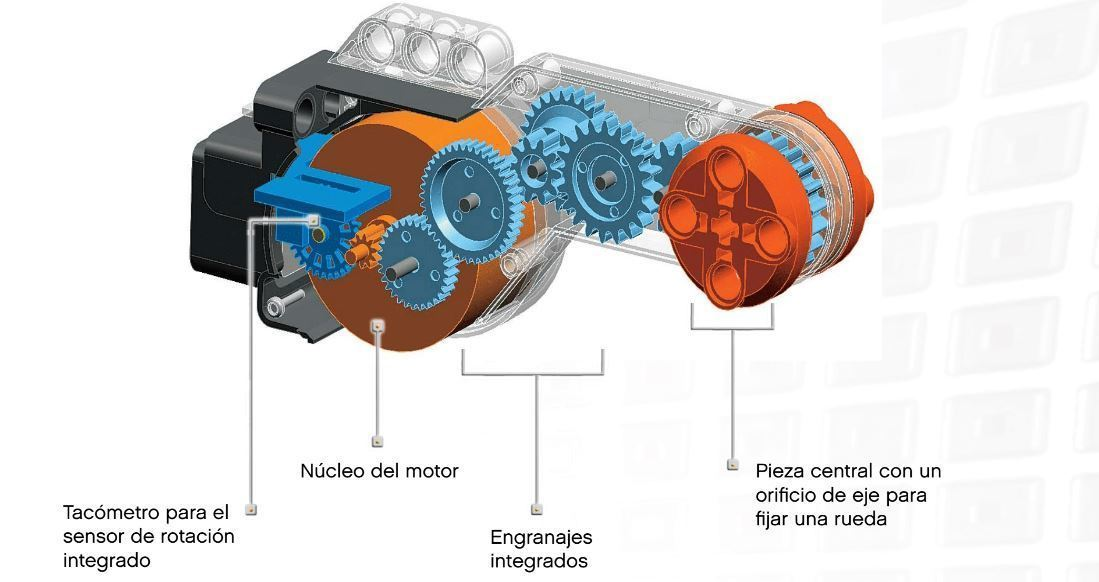
\includegraphics[scale=0.5]{graficos/motor.png}
\end{center}

Un robot diferencial es aquel que solo cuenta con dos ruedas motrices sobre un mismo eje. Cada una de estas ruedas tiene su propio motor que la hace girar perpendicular al eje que une ambas ruedas.\\

En nuestro robot hay dos ruedas (izquierda y derecha) decimos que estan unidas a por un eje ya que se encontraran paralelas al mismo nivel una de otra. Estas ruedas tienen su propio motor y encoders que miden las revoluciones. Las ruedas giran en el plano perpendicular al eje que une a ambas ruedas, cada rueda sólo puede ir hacia adelante o hacia atrás.\\

Además de las ruedas motrices, también existe una rueda loca que simplemente se utiliza para darle estabilidad al robot móvil. Esta rueda loca no es motorizada ni es importante que tenga encoders.\\

Al trabajar con el kit de robótica de LEGO Mindstorm NXT, los encoders se encuentran ya incluidos y disponibles para su uso bajo, hacemos uso de la función \textbf{MotorRotationCount}, que obtiene un valor de posición relativa respecto a una salida especifica. La salida la obtenemos en grados.

\begin{figure}[h]
  \centering
  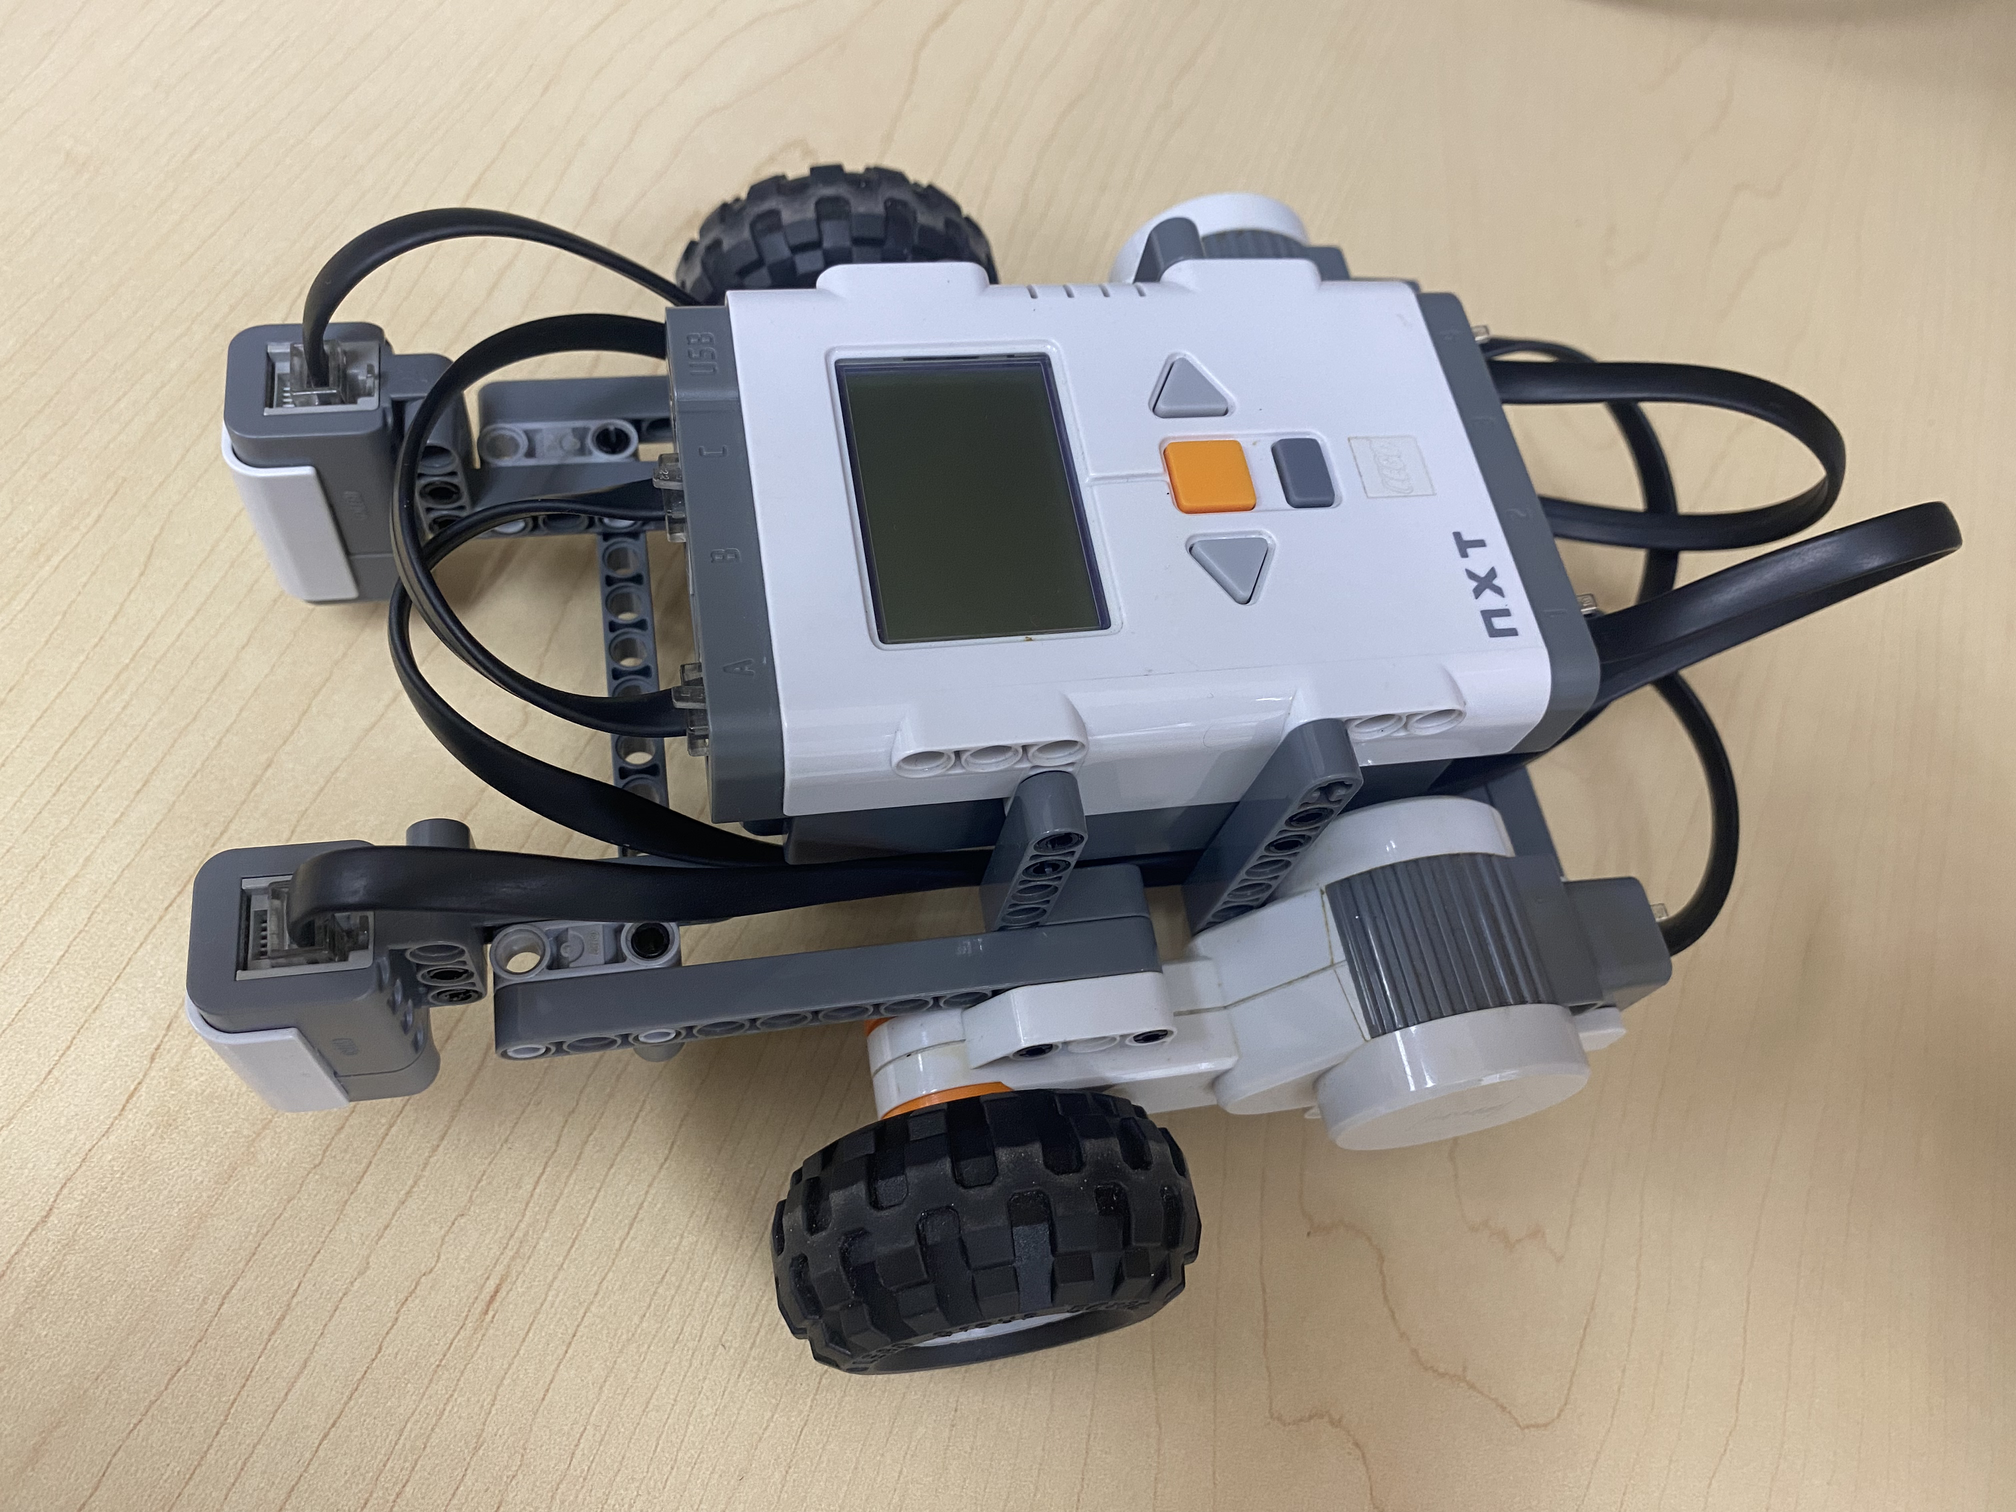
\includegraphics[scale=0.1]{graficos/robot.png}
  \caption{Robot Lego utilizado}
\end{figure}

%Describir la parte del código que se usa

\subsection{Modelo Cinemático}

El modelo cinemático es el estudio de movimiento de sistemas mecánicos sin considerar las fuerzas que afectan dicho movimiento. Para el robot móvil diferencial, su principal propósito es representar la velocidad del robot en función a las velocidades de las ruedas conjuntamente a los parámetros geométricos del robot.\\

Un robot móvil con ruedas se debe moverse sobre una superficie mediante la acción de ruedas montadas en él.
\begin{itemize}
\item El robot móvil se mueve sobre una superficie plana horizontal, es decir es constante
\item Los ejes de referencia son perpendiculares al suelo
\item No existen elementos flexibles en la estructura del robot
\item El contacto entre cada rueda y el suelo se reduce a un solo punto
\item No existe deslizamiento
\end{itemize}

El modelado del robot se puede representar como la siguiente imágen

\begin{figure}[h]
  \centering
  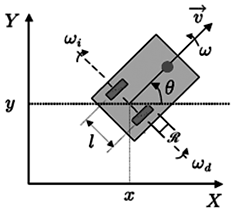
\includegraphics[scale=0.6]{graficos/odometria.png}
  \caption{Modelo Robot}
\end{figure}

Donde:
\begin{itemize}
\item \textbf{$\theta$}: Ángulo de orientación del robot
\item \textbf{$\omega_{l}$}: Velocidad angular rueda izquierda
\item \textbf{$\omega_{r}$}: Velocidad angular rueda derecha
\item \textbf{$\vec{v_{l}}$}: Velocidad rueda izquierda
\item \textbf{$\vec{v_{r}}$}: Velocidad rueda derecha
\item \textbf{$l$}: Distancian entre las dos ruedas medidas haciendo referencia a su punto de apoyo
\item $R$: Radio del robot
\item $x,y$: Posición x,y en el plano
\item \textbf{$D_{l}$}: Distancia recorrida rueda izquierda
\item \textbf{$D_{r}$}: Distancia recorrida rueda derecha
\item \textbf{$Dc$}: Distancia recorrida por el robot
\end{itemize}

Partiendo de la ubicación del centro de nuestro robot, considerando el punto medio como el punto que corta entre la línea de acción l y una perpendicular a la rueda motriz, considerando un robot móvil de direccionamiento diferencial no holonómico que se mueve en un plano horizontal, se describe su cinemática con las ecuaciones:

\[ x' = \frac{dx}{dt} = v*cos \theta \qquad y' = \frac{dy}{dt} = v*sen \theta \qquad \dot{\theta} = \omega \]

\[ p = \begin{bmatrix}
  \dot{x}\\
  \dot{y}\\
  \dot{\theta}
\end{bmatrix}\]

es el vector que nos indica la posición y orientación del robot

Partiendo del gráfico del modelo del robot, podemos observar que existe una relaciónes donde hacemos uso de funciones trigonometricas \textbf{Seno y Coseno}, para conocer la posición x,y de nuestro robot a medida que recopilamos datos del encoder. Pero antes debemos contar con el vector resultante de nuestro robot con los datos conocidos de la rueda izquierda y derecha.\\

Distancia Derecha - partiendo de las mediciones de rotación obtenidas en grados, las convertimos a radianes\\
\[ D_{L} = radio * (Lectura Rueda Izquierda * (\frac{\pi}{180})) \qquad D_{R} = radio * (Lectura Rueda Derecha * (\frac{\pi}{180})) \]

La distancia recorrida por nuestro robot será el promedio de ambas distancias:
\[D_{ROBOT} = \frac{(D_{R}+D_{L})}{2}\]

Una vez obtenidos los parámetros anteriores, podemos calcular nuestro ángulo de giro $\omega$
\[\omega = \frac{(DR-DL)}{\mbox{longitud entre ruedas}} \]

Nuestro ángulo de giro obtenido de la ecuación anterior nos dan los grados en radianes, para obtenerlo en grados multiplicamos por $\frac{180}{\pi}$, de esta forma podremos hacer uso de las primeras ecuaciones para conocer las nuevas coordenadas x,y en el plano.

\[ x = x + \mbox{Distancia Robot} * \frac{cos(\theta)}{100} \qquad y = y + \mbox{Distancia Robot} * \frac{sen(\theta)}{100} \]

\subsection{Programa}

El programa del odómetro debe consistir en las siguientes fases dentro de un ciclo infinito

\begin{itemize}
\item Leer tacómetros
\item Comparar con lectura anterior
\item Calcular las diferencias $\Delta X$
\item Calcular las diferencias $\Delta Y$
\item Calcular las diferencias $\Delta \theta$
\item Actualizar odómetro $(X+\Delta X, Y+\Delta Y, \theta + \Delta \theta)$
\item Actualizar mediciones
\end{itemize}

\subsection{Pseudocódigo}

Durante la realización del odómetro, el interprete no soporta asignaciones con expresiones largas, es por eso que en el código la asignación para las nuevas coordenadas x,y se dividieron para así contar con los datos correctos.

\begin{algorithm}
  \caption{Odómetro}\label{alg:two}
  Leer tacometros\;
  Comparar con lectura anterior\;
  \If{supera umbral}{
    $\Delta X \gets X + \Delta X$\; %\Comment*[r]{MAX iter for exploration, if no solution}
    $\Delta Y \gets Y + \Delta Y$\;
    $\Delta \Theta \gets \Theta + \Delta \Theta$\; 
    Actualizar Odómetro\;
    Actualizar Tacometro\;
  }
  Wait(50ms)\;
\end{algorithm}

La implementación quedará dentro de una tarea (task), ya que el kit de LEGO NXT haciendo uso de NXC soporta multiples hilos de ejecución de tareas. Se incluyen más tareas como un seguidor de linea básico, e ir mostrando el desplazamiento del robot en la pantalla del ladrillo LEGO. La ejecución de los hilos la realiza el hilo principal con ayuda un organizador de una lista de tareas \textbf{Precedes} con el siguiente orden: \\
\textbf{Precedes(odometria,sigue\_lineas,make\_draw)\;} 

\subsection{Pruebas}

Durante las pruebas se pueden observar errores, dichos errores sistemáticos los podemos considerar agenos al modelo dichos errores pueden ser variados como:
\begin{itemize}
\item Los diametros de las ruedas no son iguales
\item Medida errorena de los diámetros de las ruedas
\item Mal alineación de las ruedas
\item Irregularidad del terreno
\item Derrape, patinaje
\end{itemize}

Los errores no sistemáticos los podemos corregir con una calibración. A continuación se muestran tres erres de tres corridas diferentes.

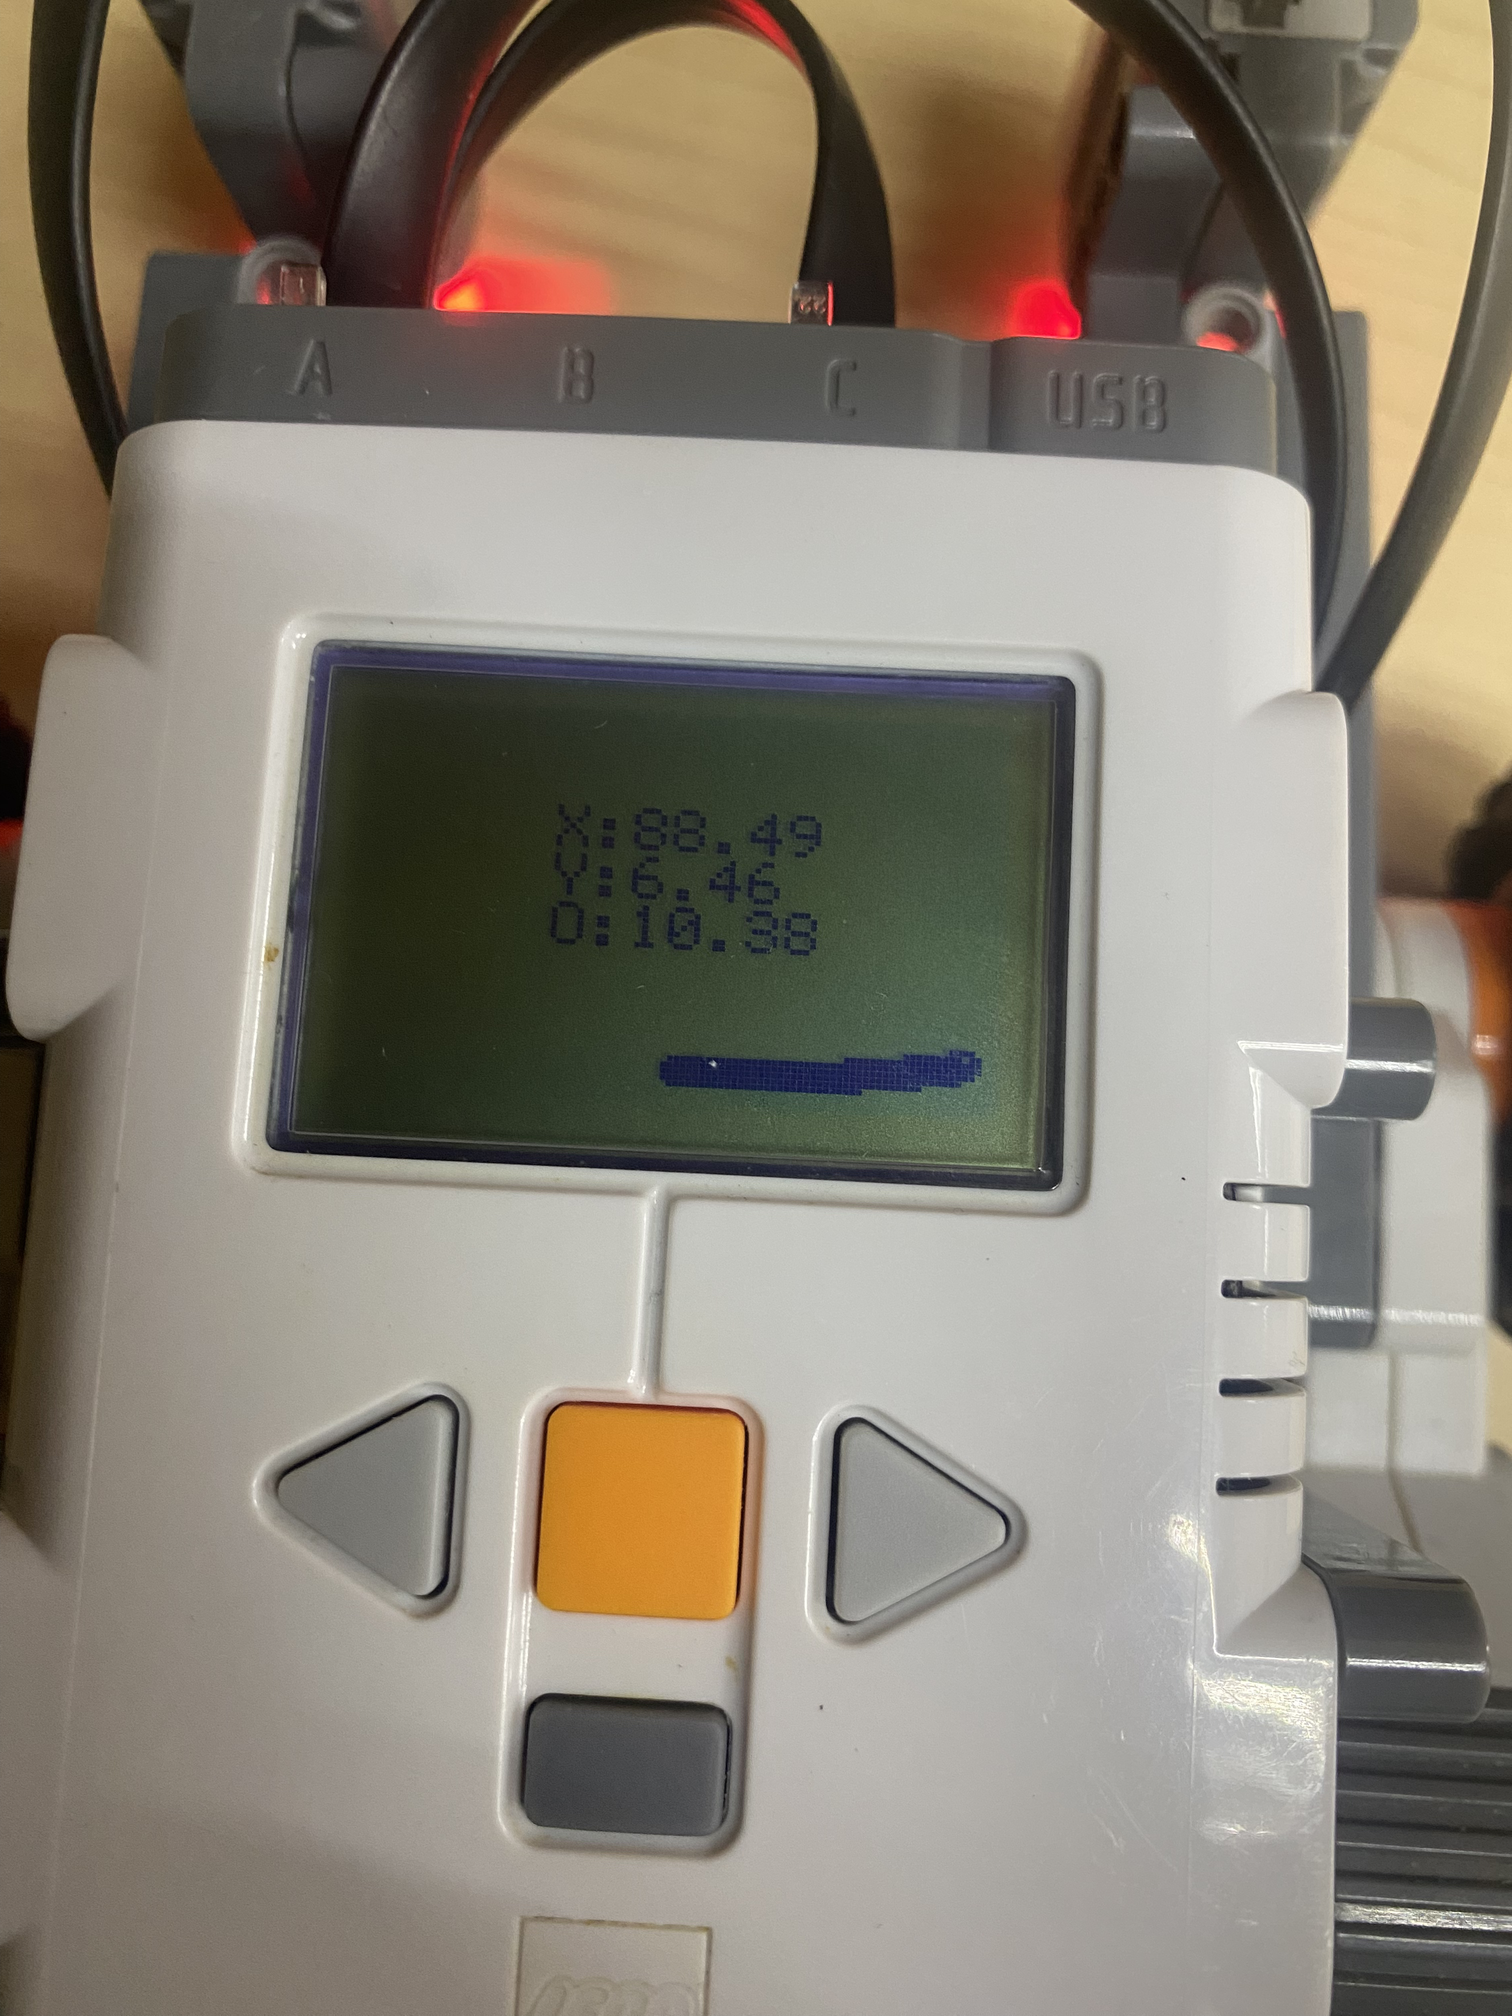
\includegraphics[scale=0.09]{graficos/error1.png}
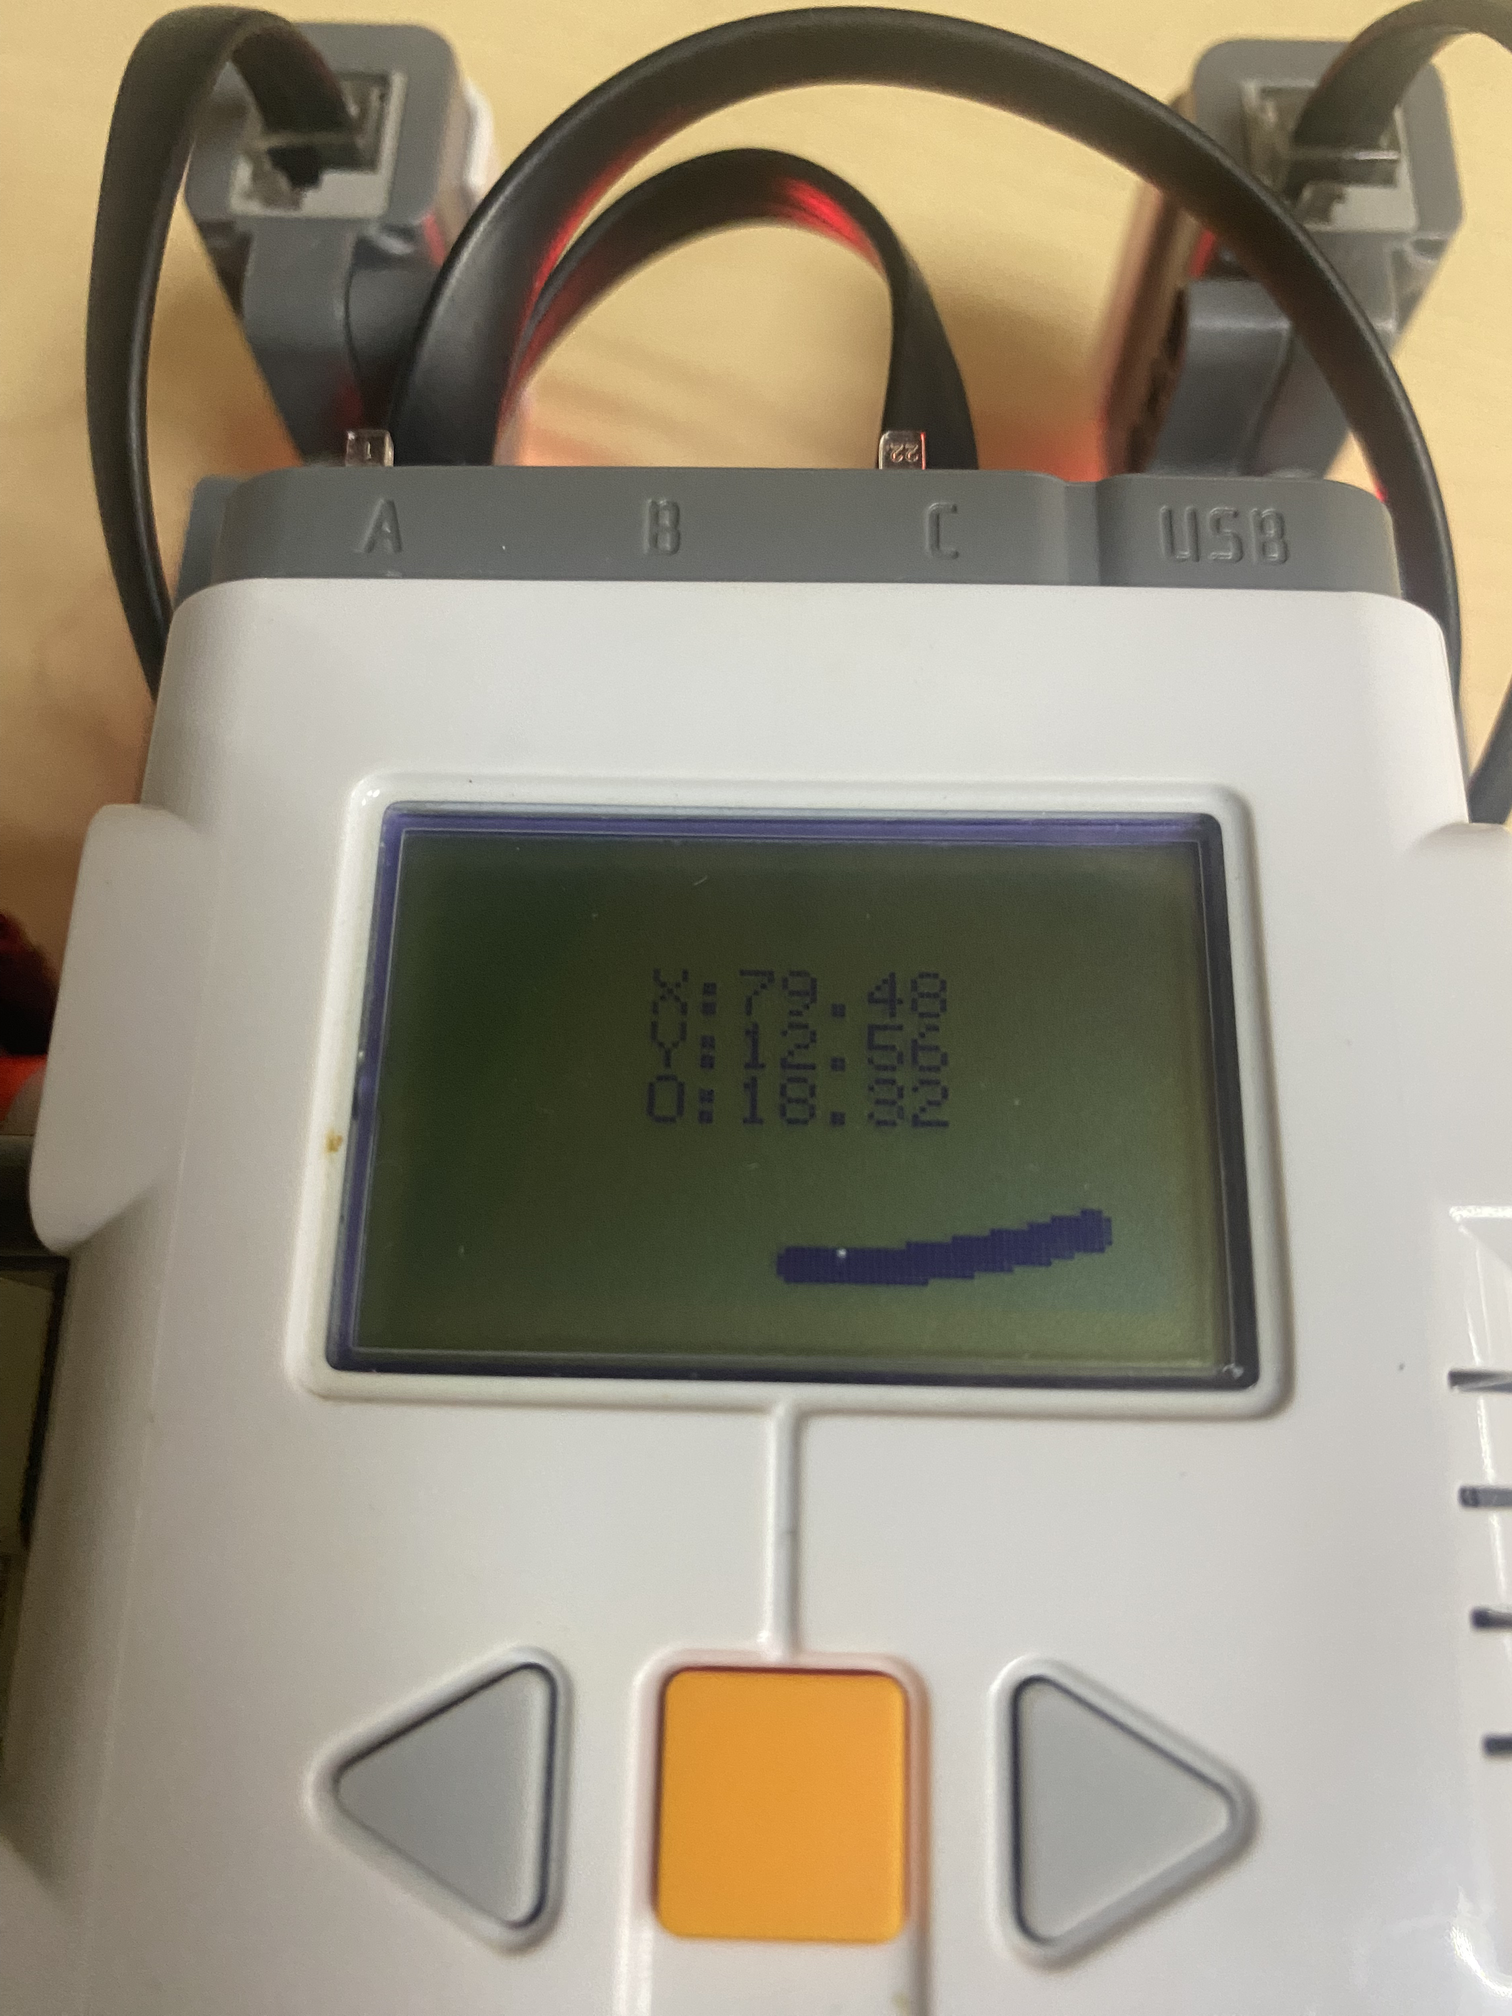
\includegraphics[scale=0.09]{graficos/error2.png}
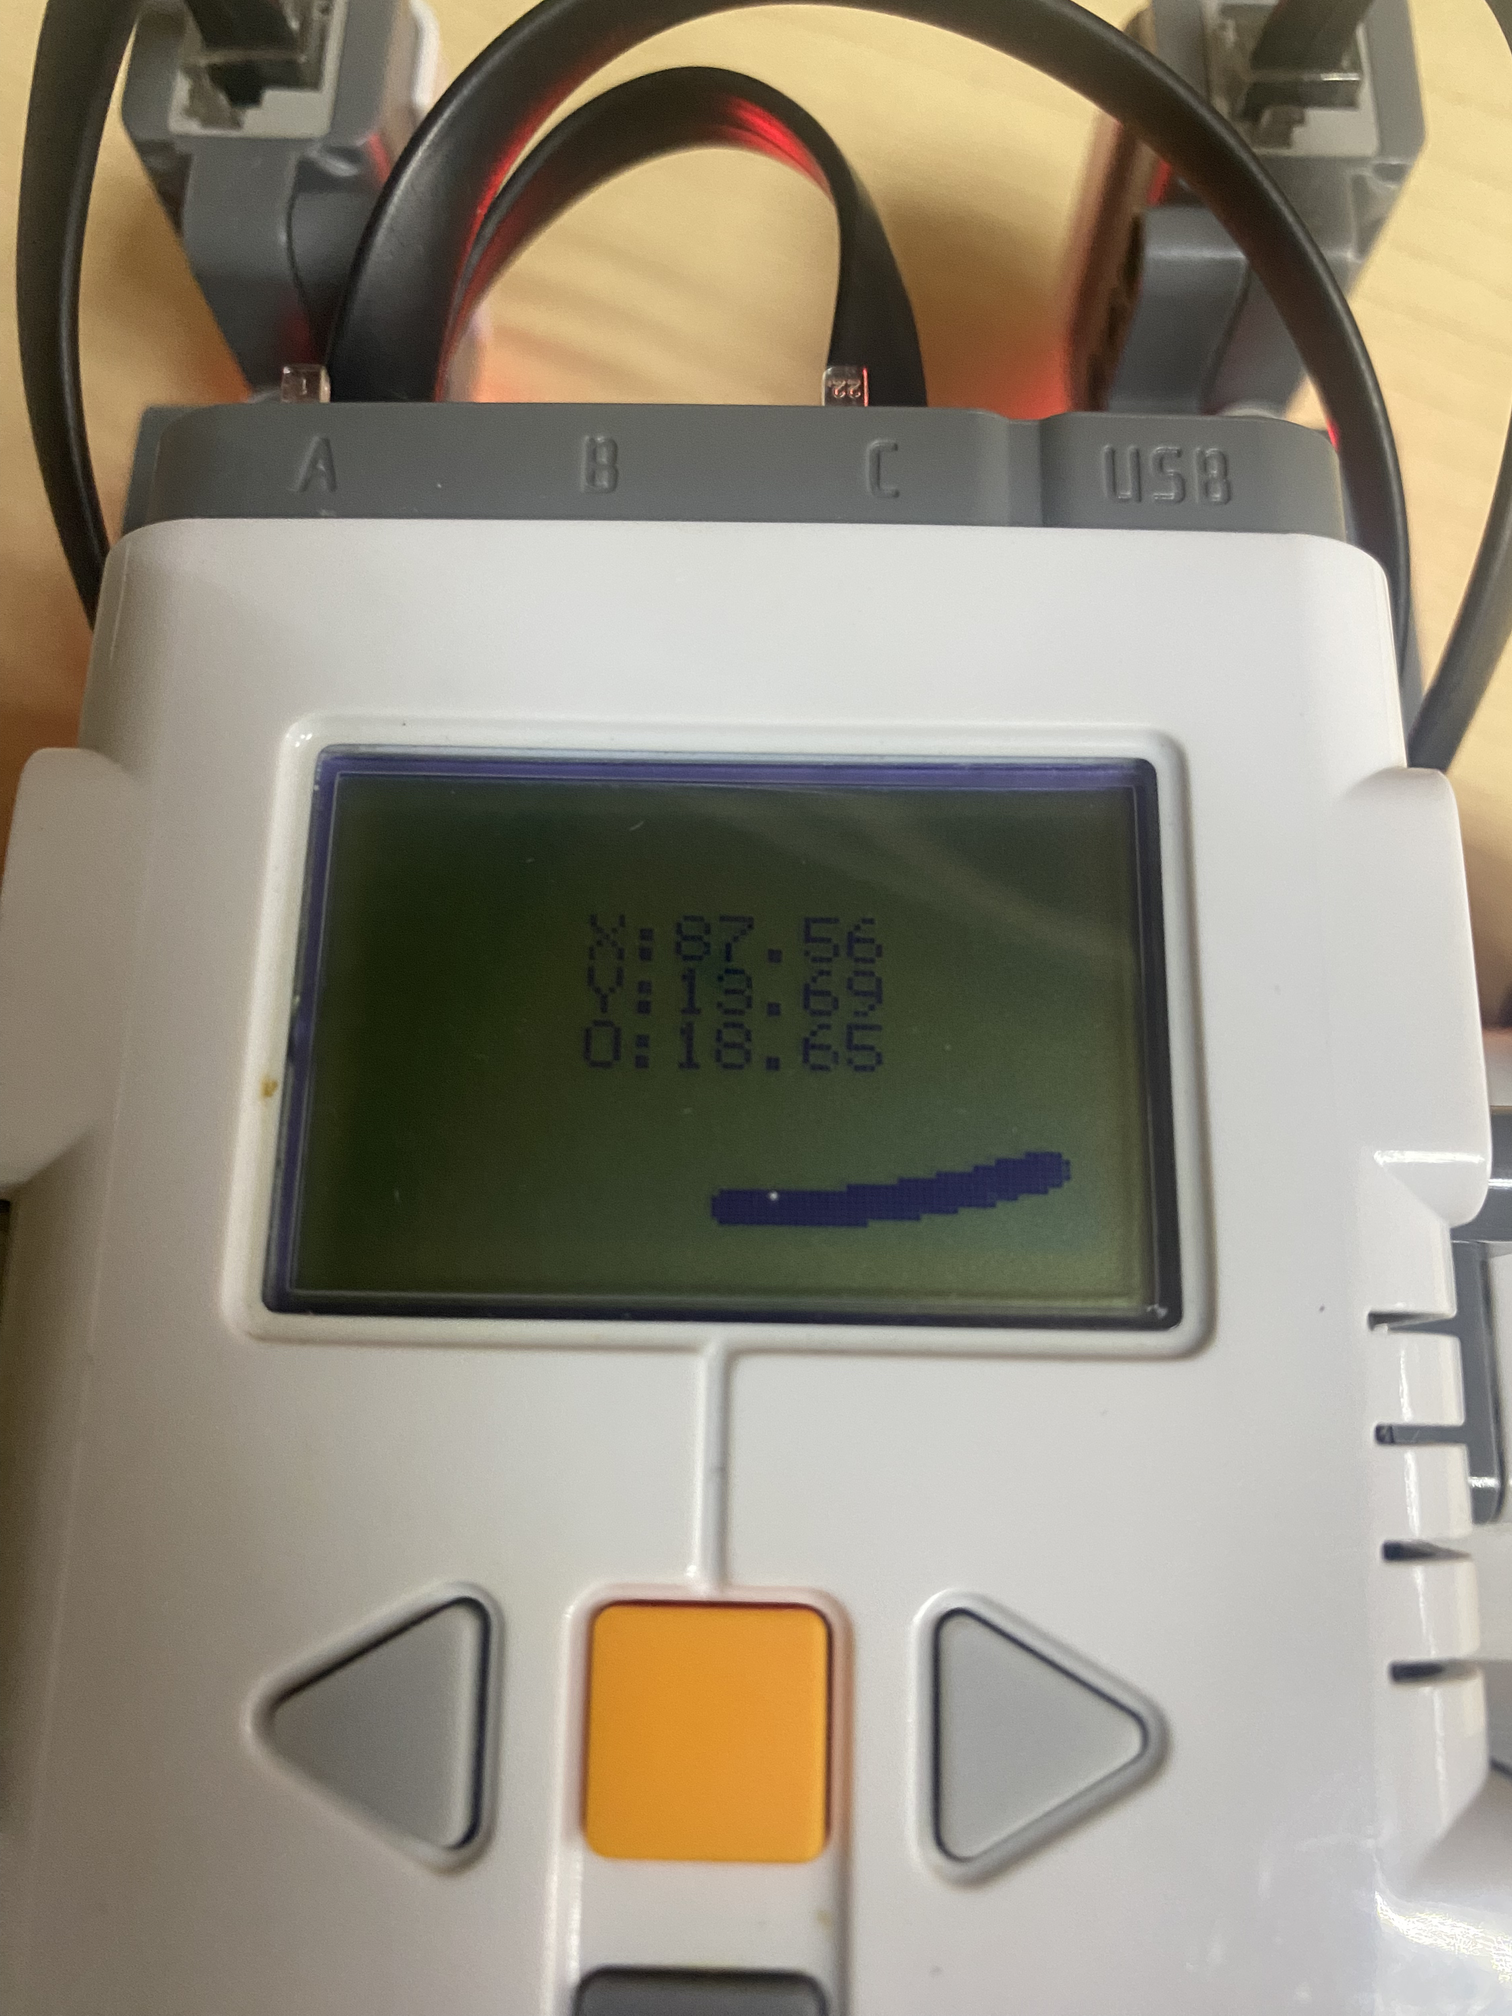
\includegraphics[scale=0.09]{graficos/error3.png}

En la primera imágen después de un desplazamiento aproximado de 86 cm, los datos de desplazamiento del robot fueron: 88.49 cm y una inclinación de 10.38$^{\circ}$

\begin{figure}[!hb]
  \centering
  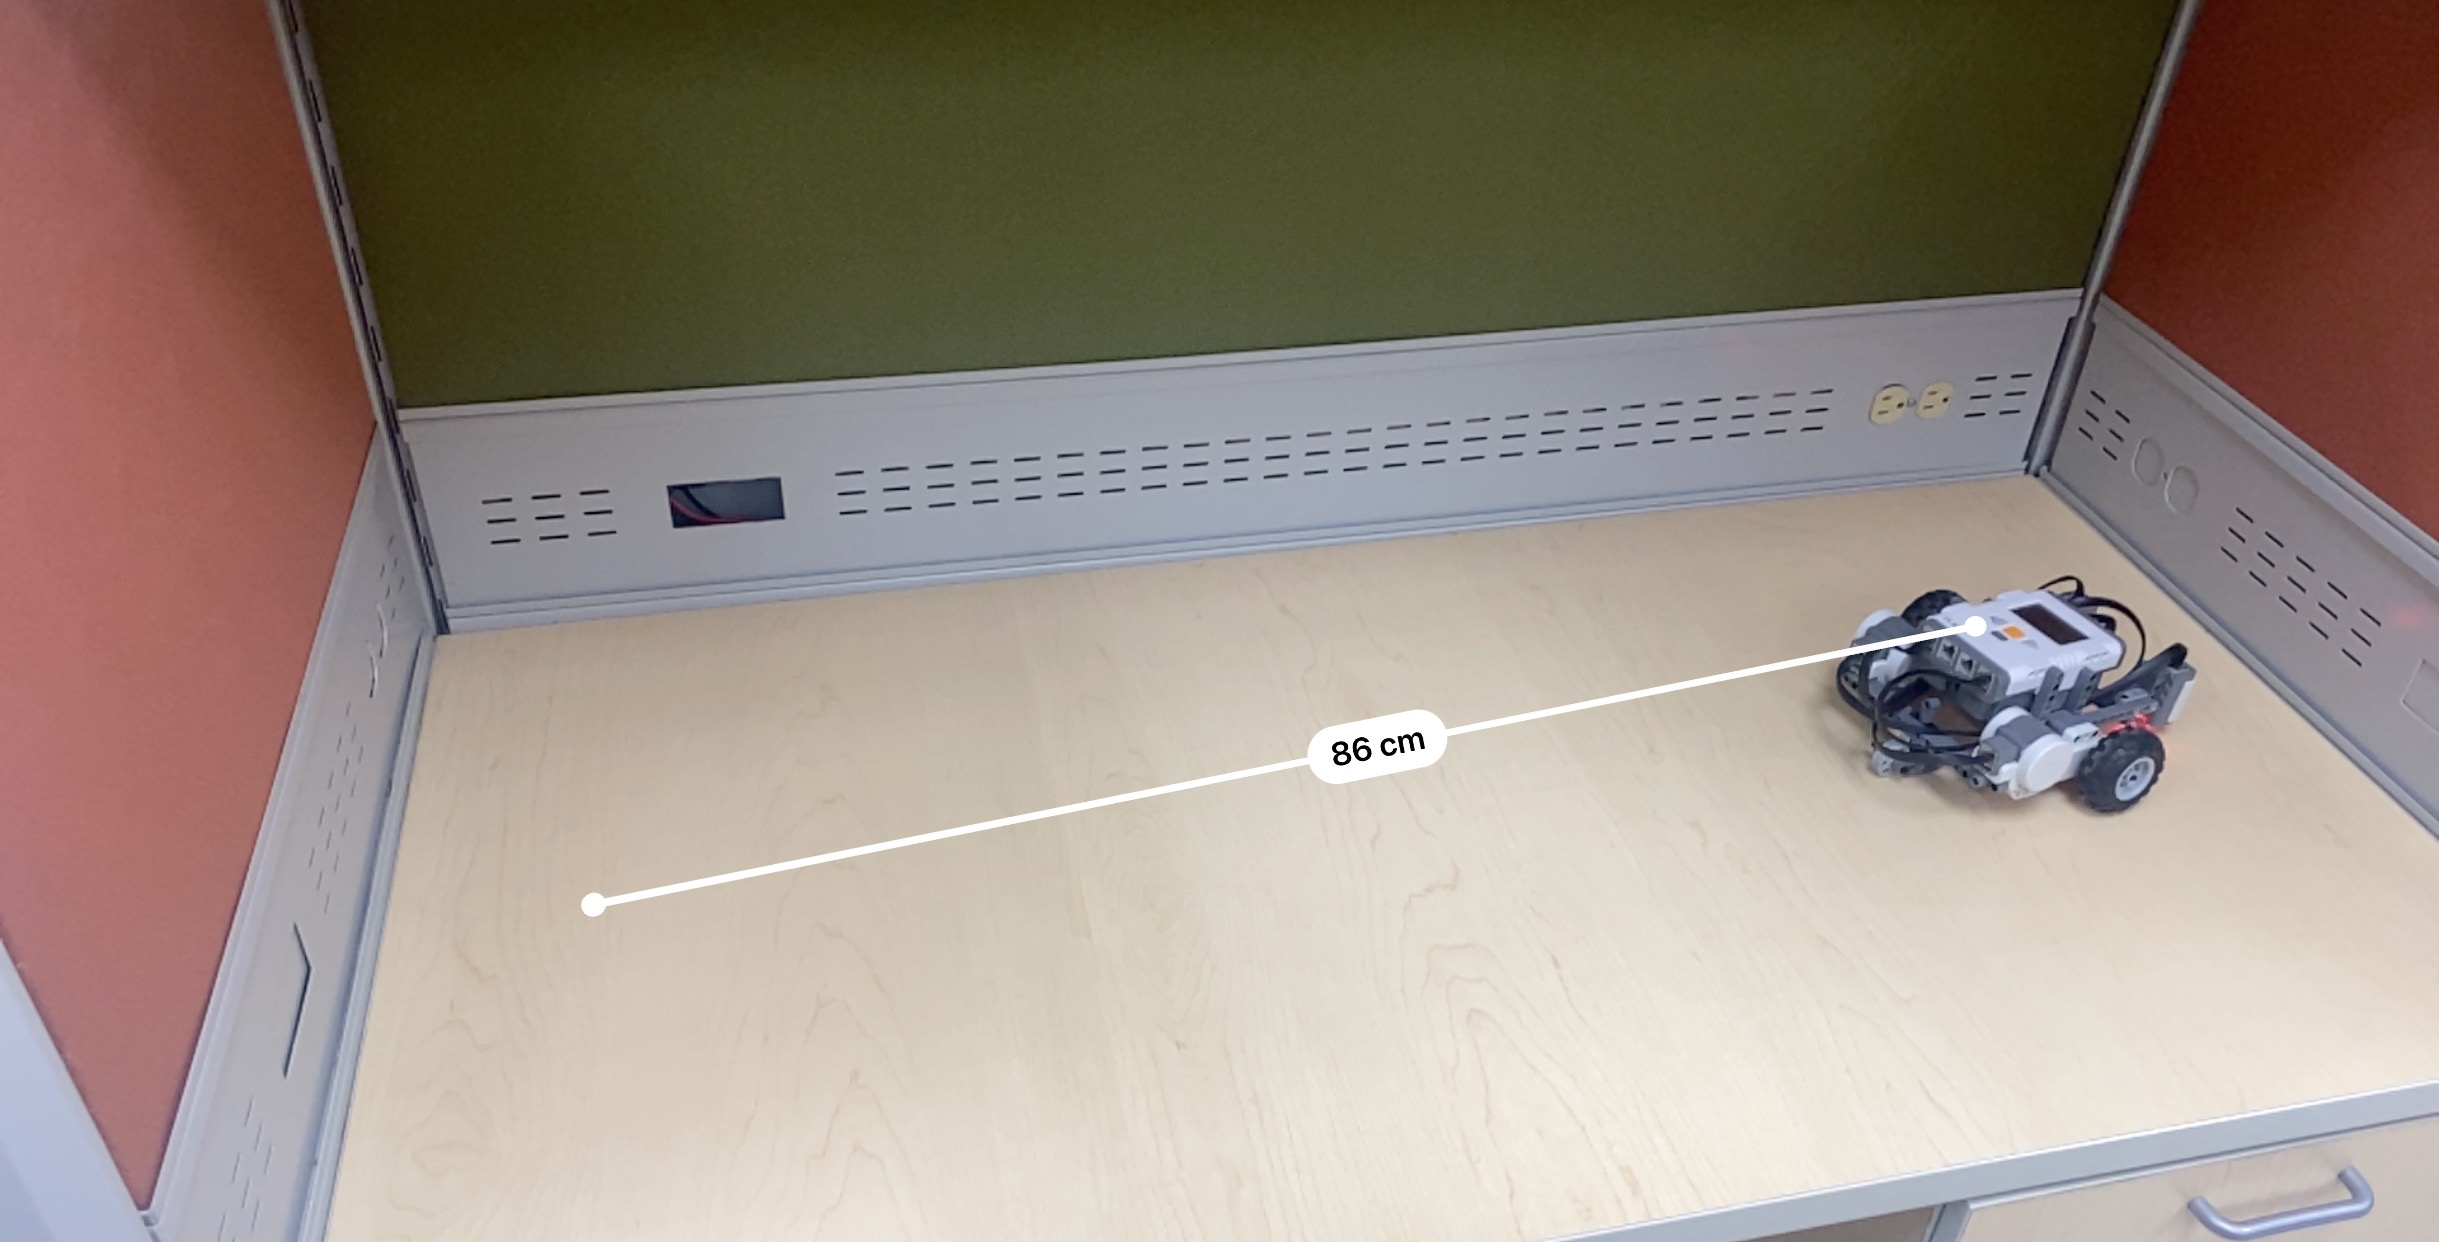
\includegraphics[scale=0.18]{graficos/prueba1.JPG}
\end{figure}

\newpage
En la segunda prueba después de un desplazamiento aproximado de 75 cm, los datos de desplazamiento del robot fueron: 79.48 cm y una inclinación de 18.32$^{\circ}$
\begin{figure}[!hb]
  \centering
  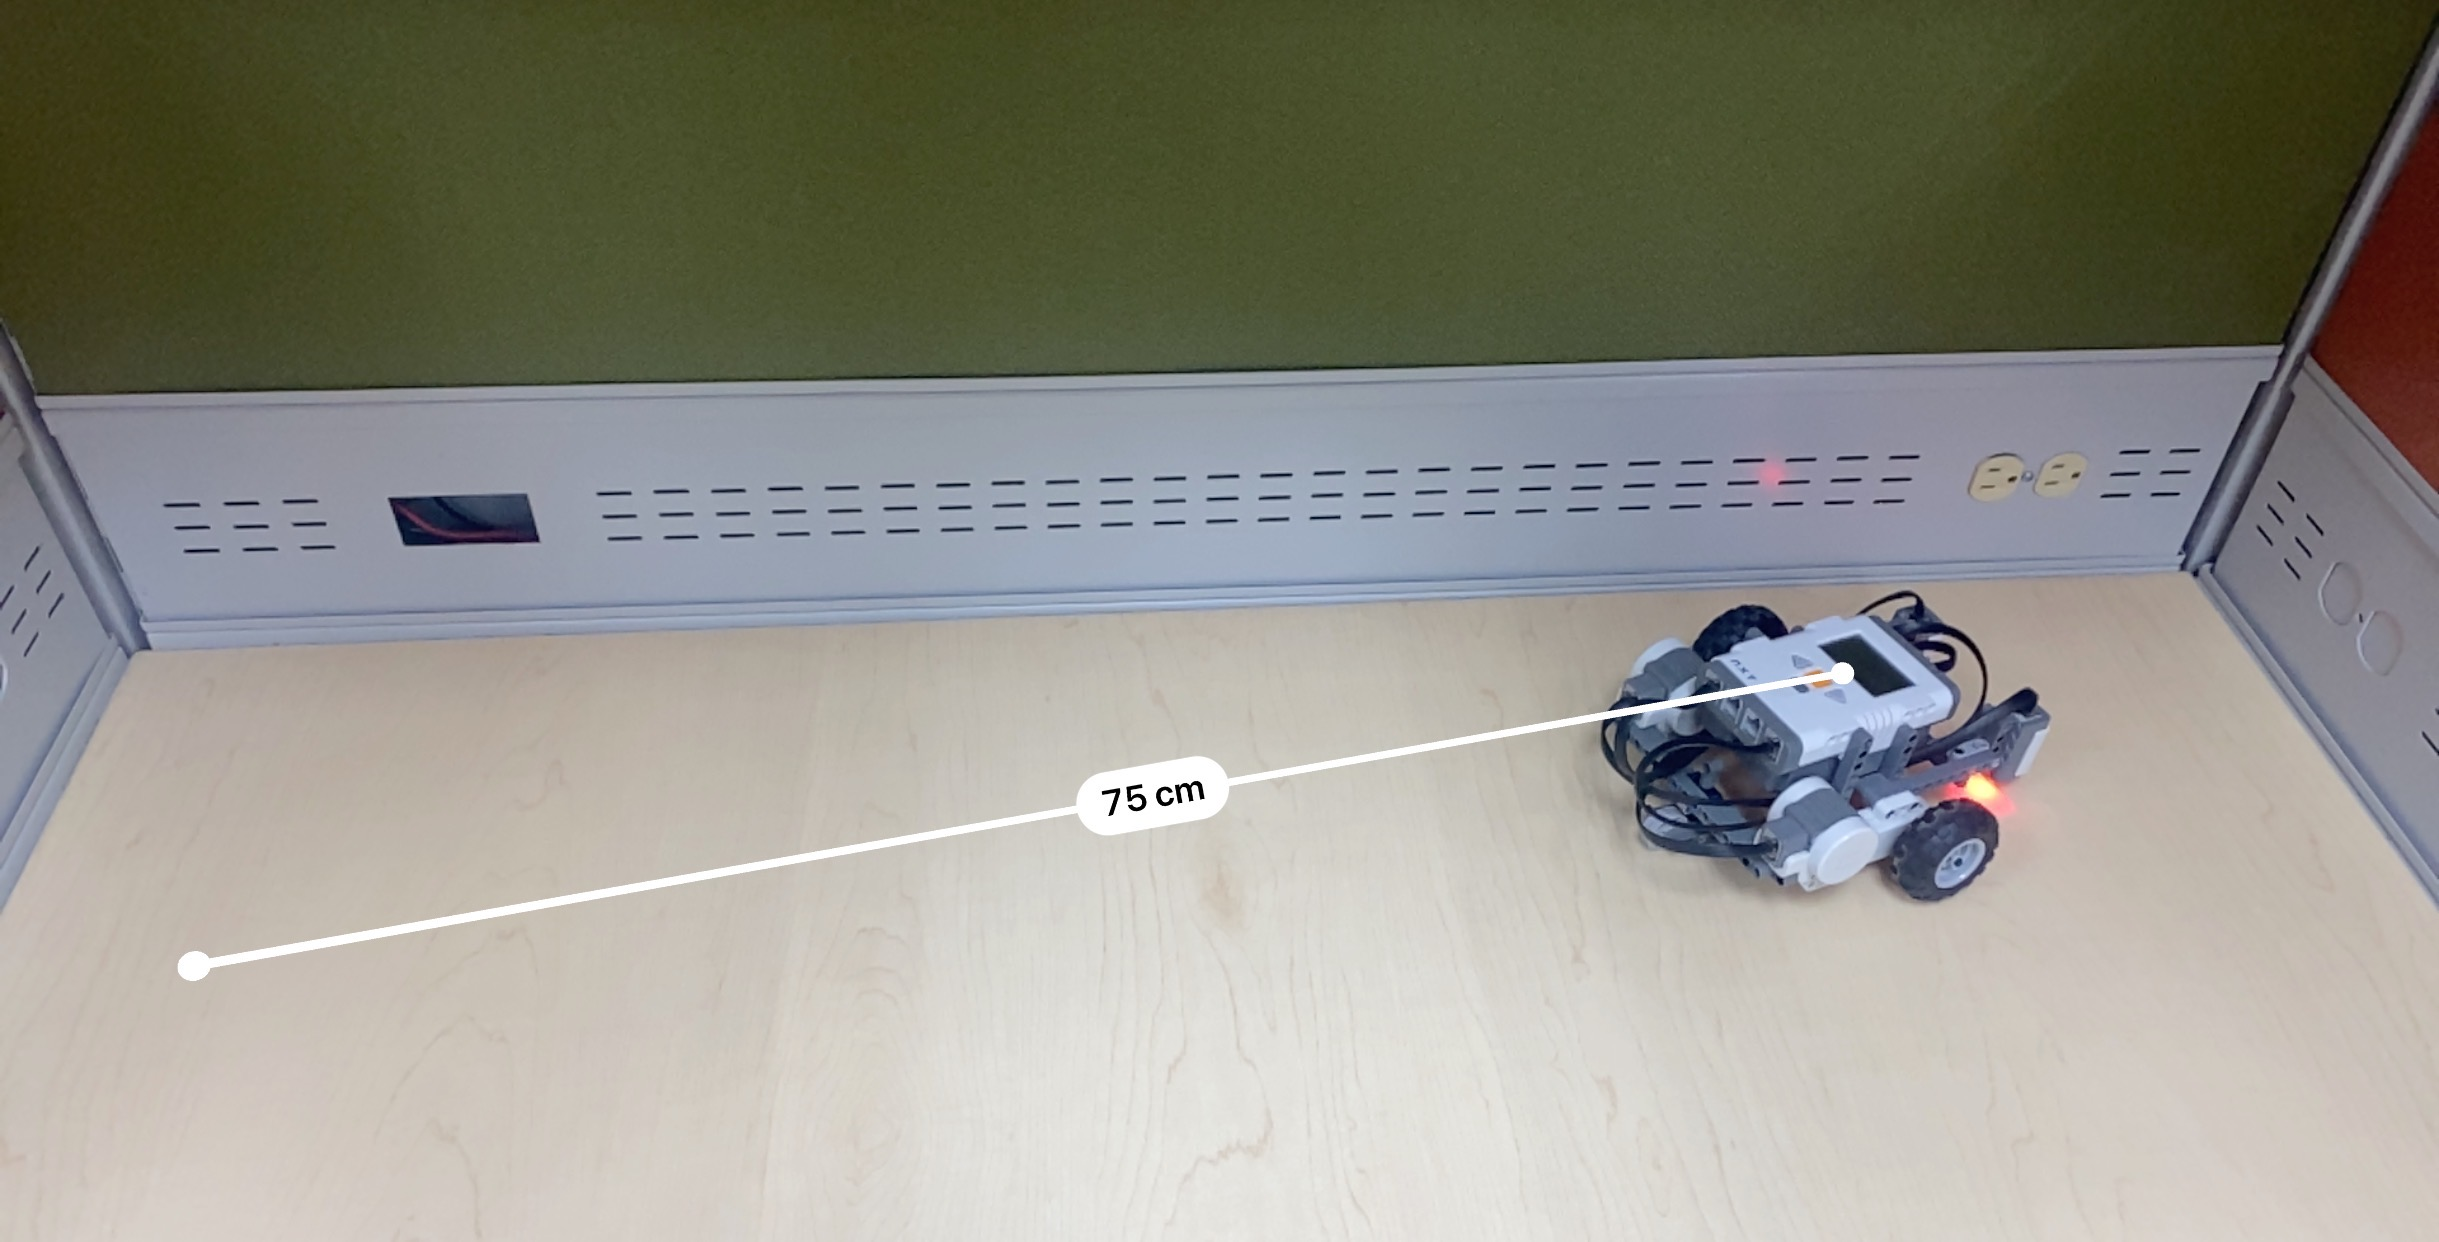
\includegraphics[scale=0.18]{graficos/prueba2.JPG}
\end{figure}

En la tercera prueba después de un desplazamiento aproximado de 86 cm, los datos de desplazamiento del robot fueron: 87.56 cm y una inclinación de 18.65$^{\circ}$

\begin{figure}[!hb]
  \centering
  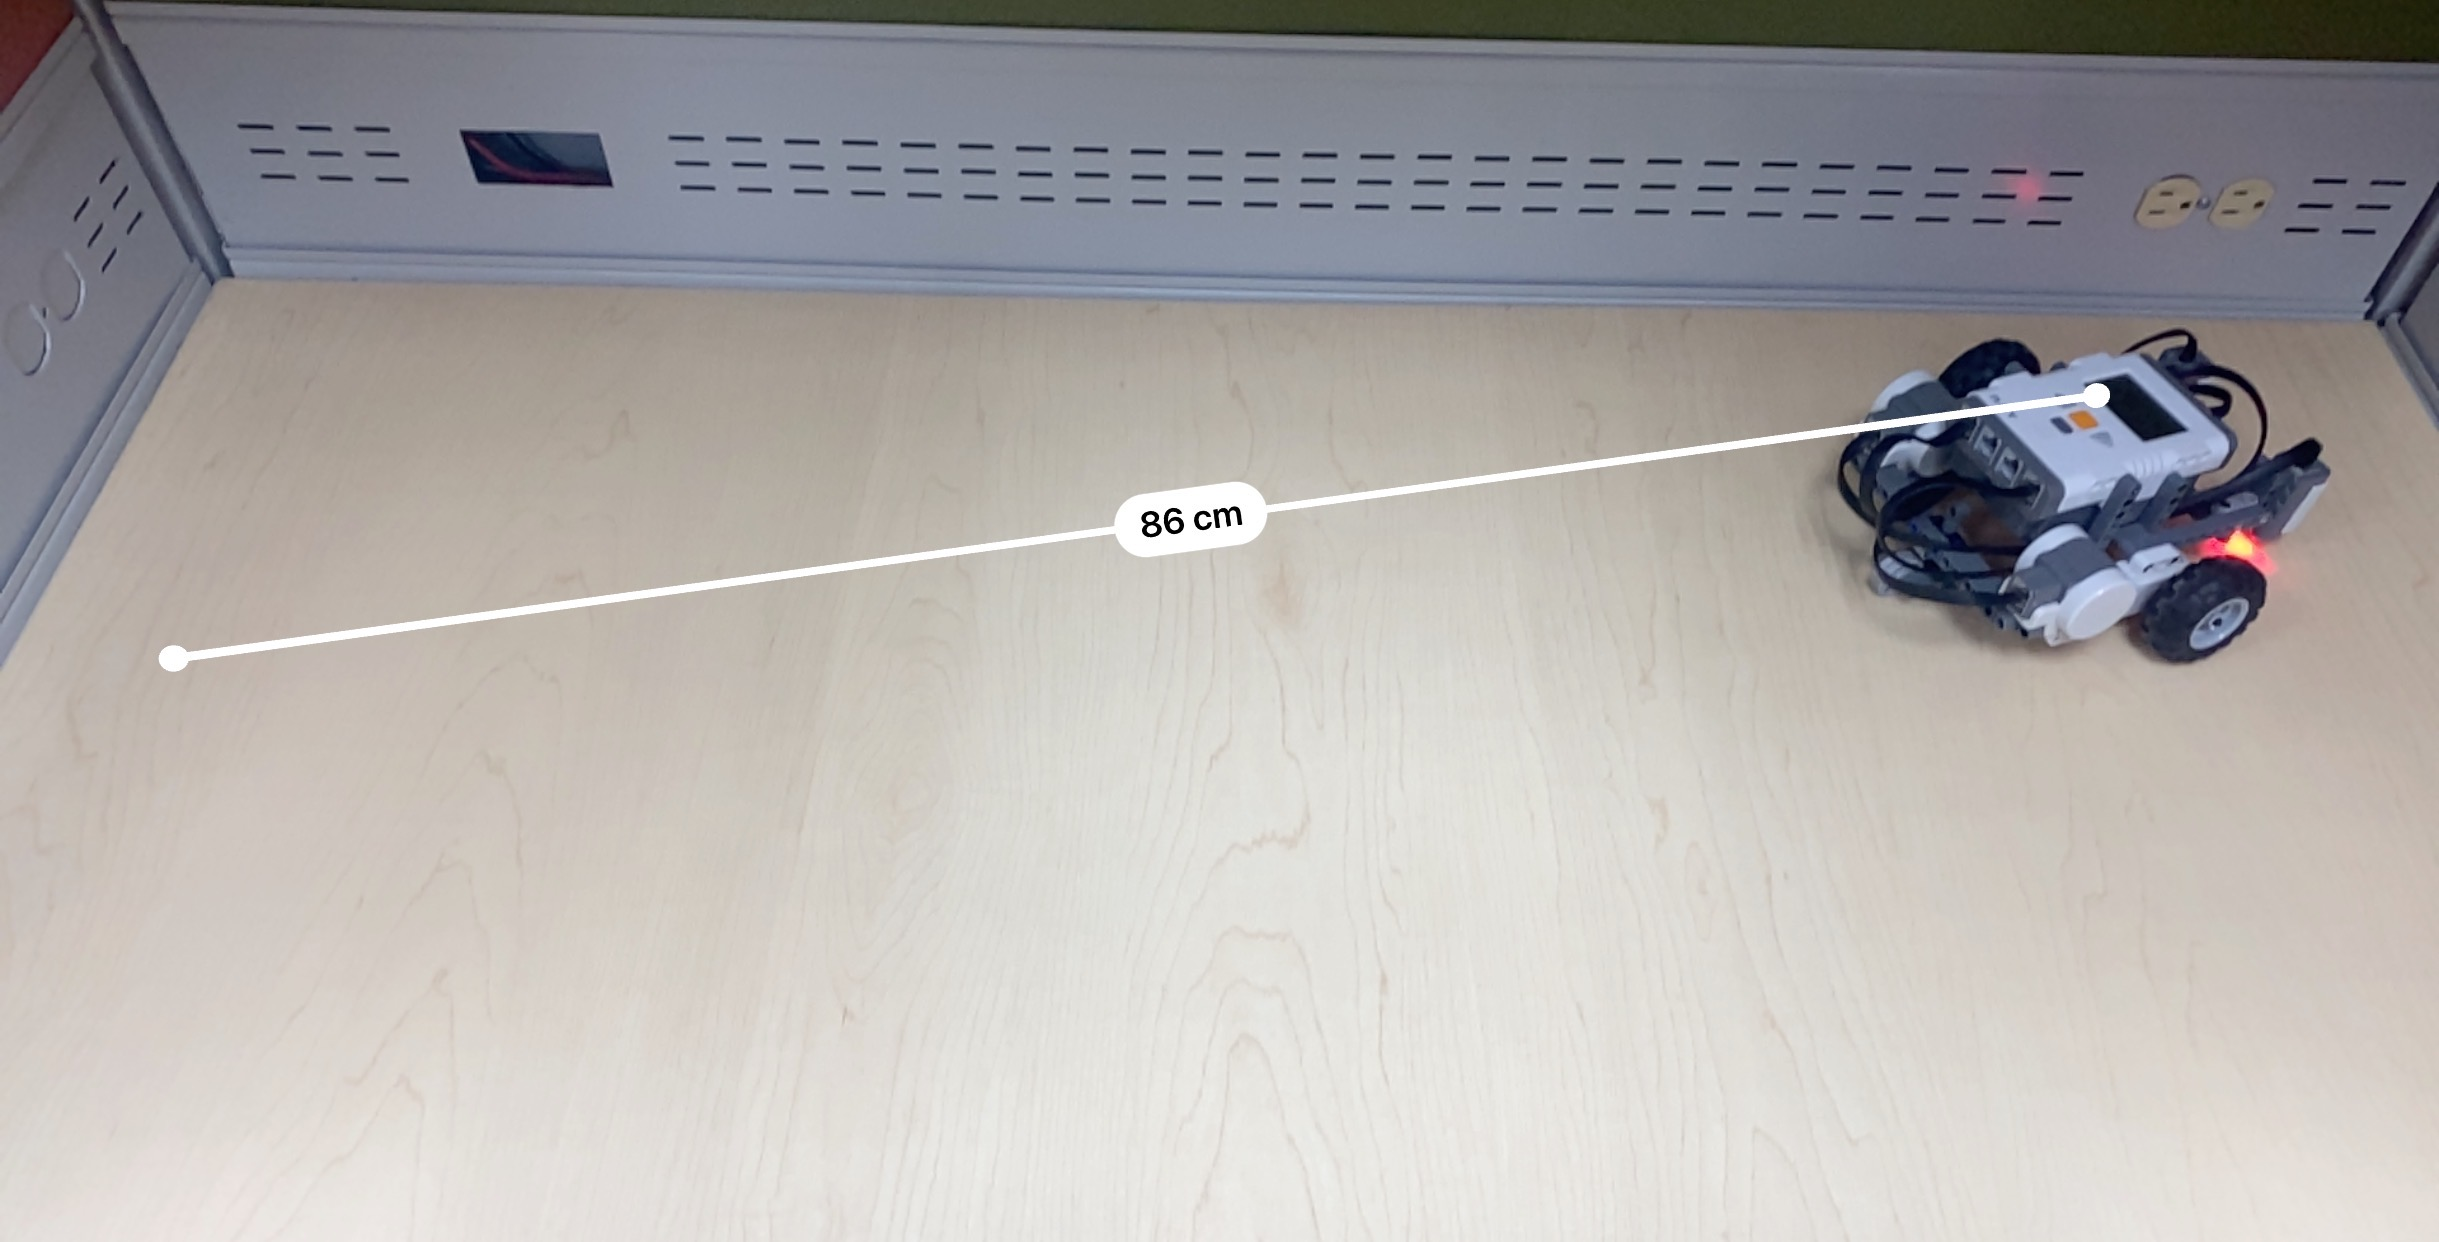
\includegraphics[scale=0.18]{graficos/prueba3.JPG}
\end{figure}

\newpage
\subsection{Prueba con el siguelineas}

Al tener calibrado nuestras mediciones del odómetro, lo integramos dentro de la rutina de sigue-líneas.

\begin{figure}[!hb]
  \centering
  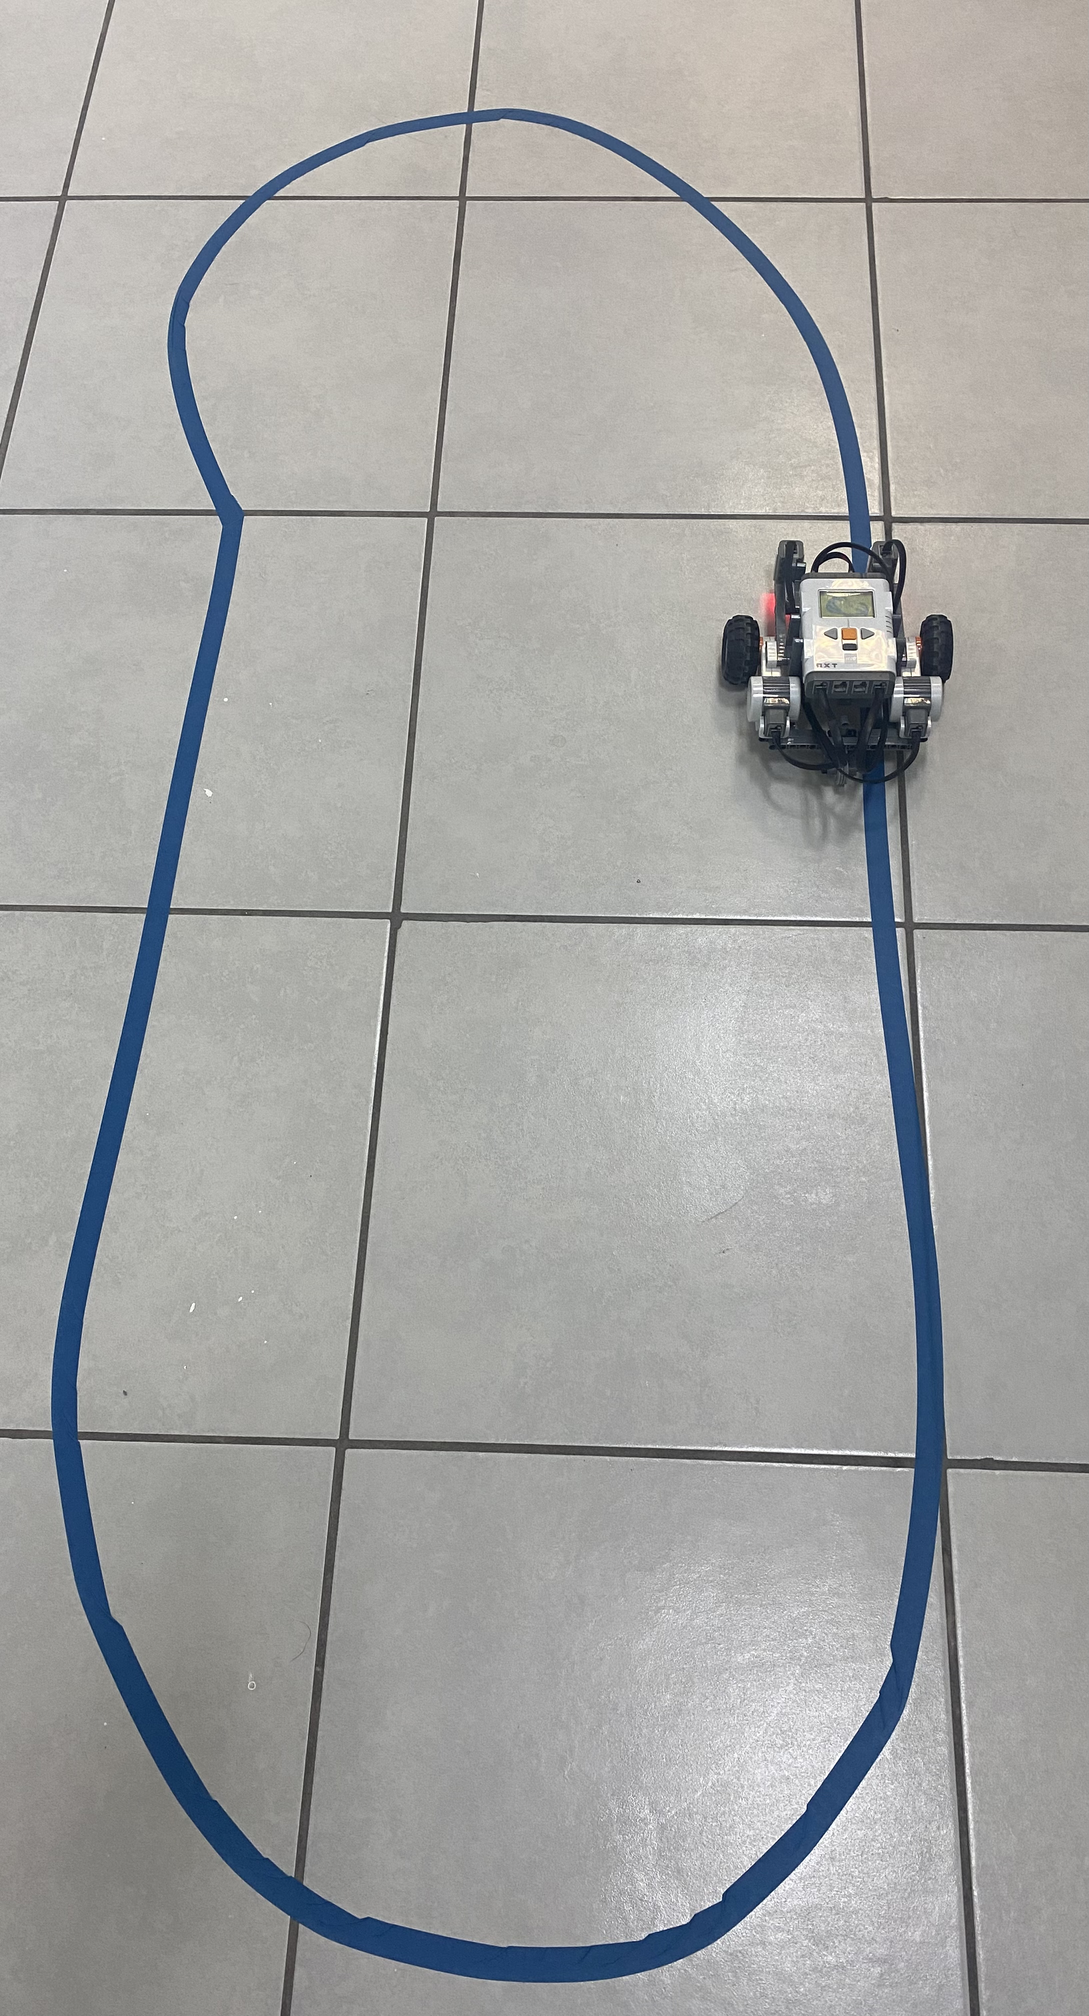
\includegraphics[angle=90,scale=0.2]{graficos/path_robot.png}
\end{figure}
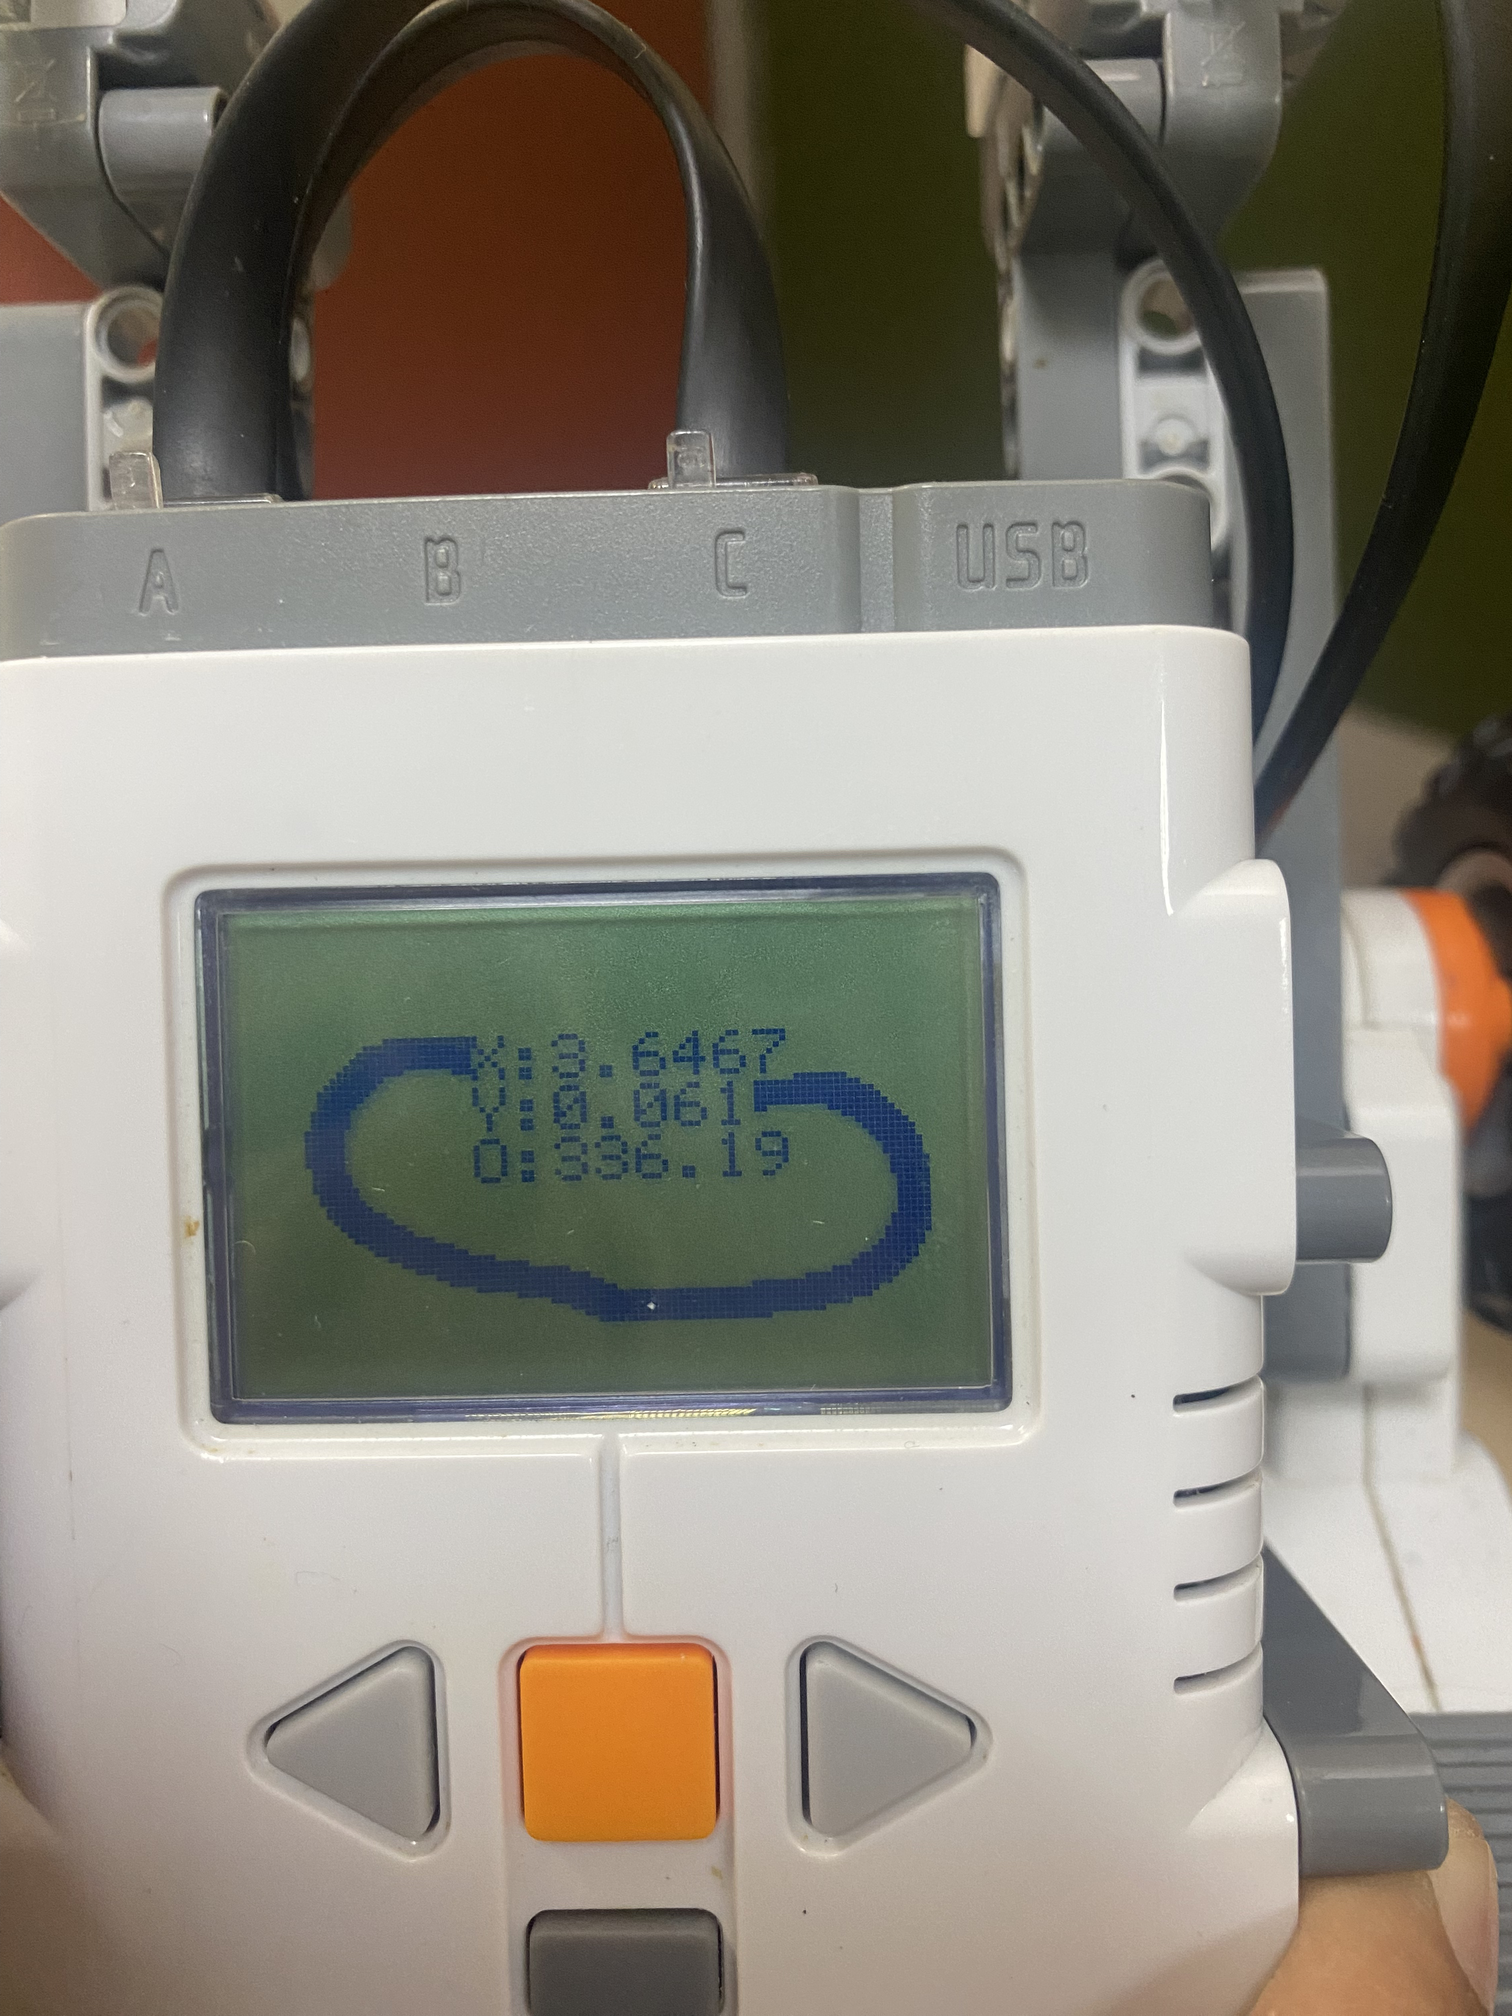
\includegraphics[scale=0.09]{graficos/corrida1.png}
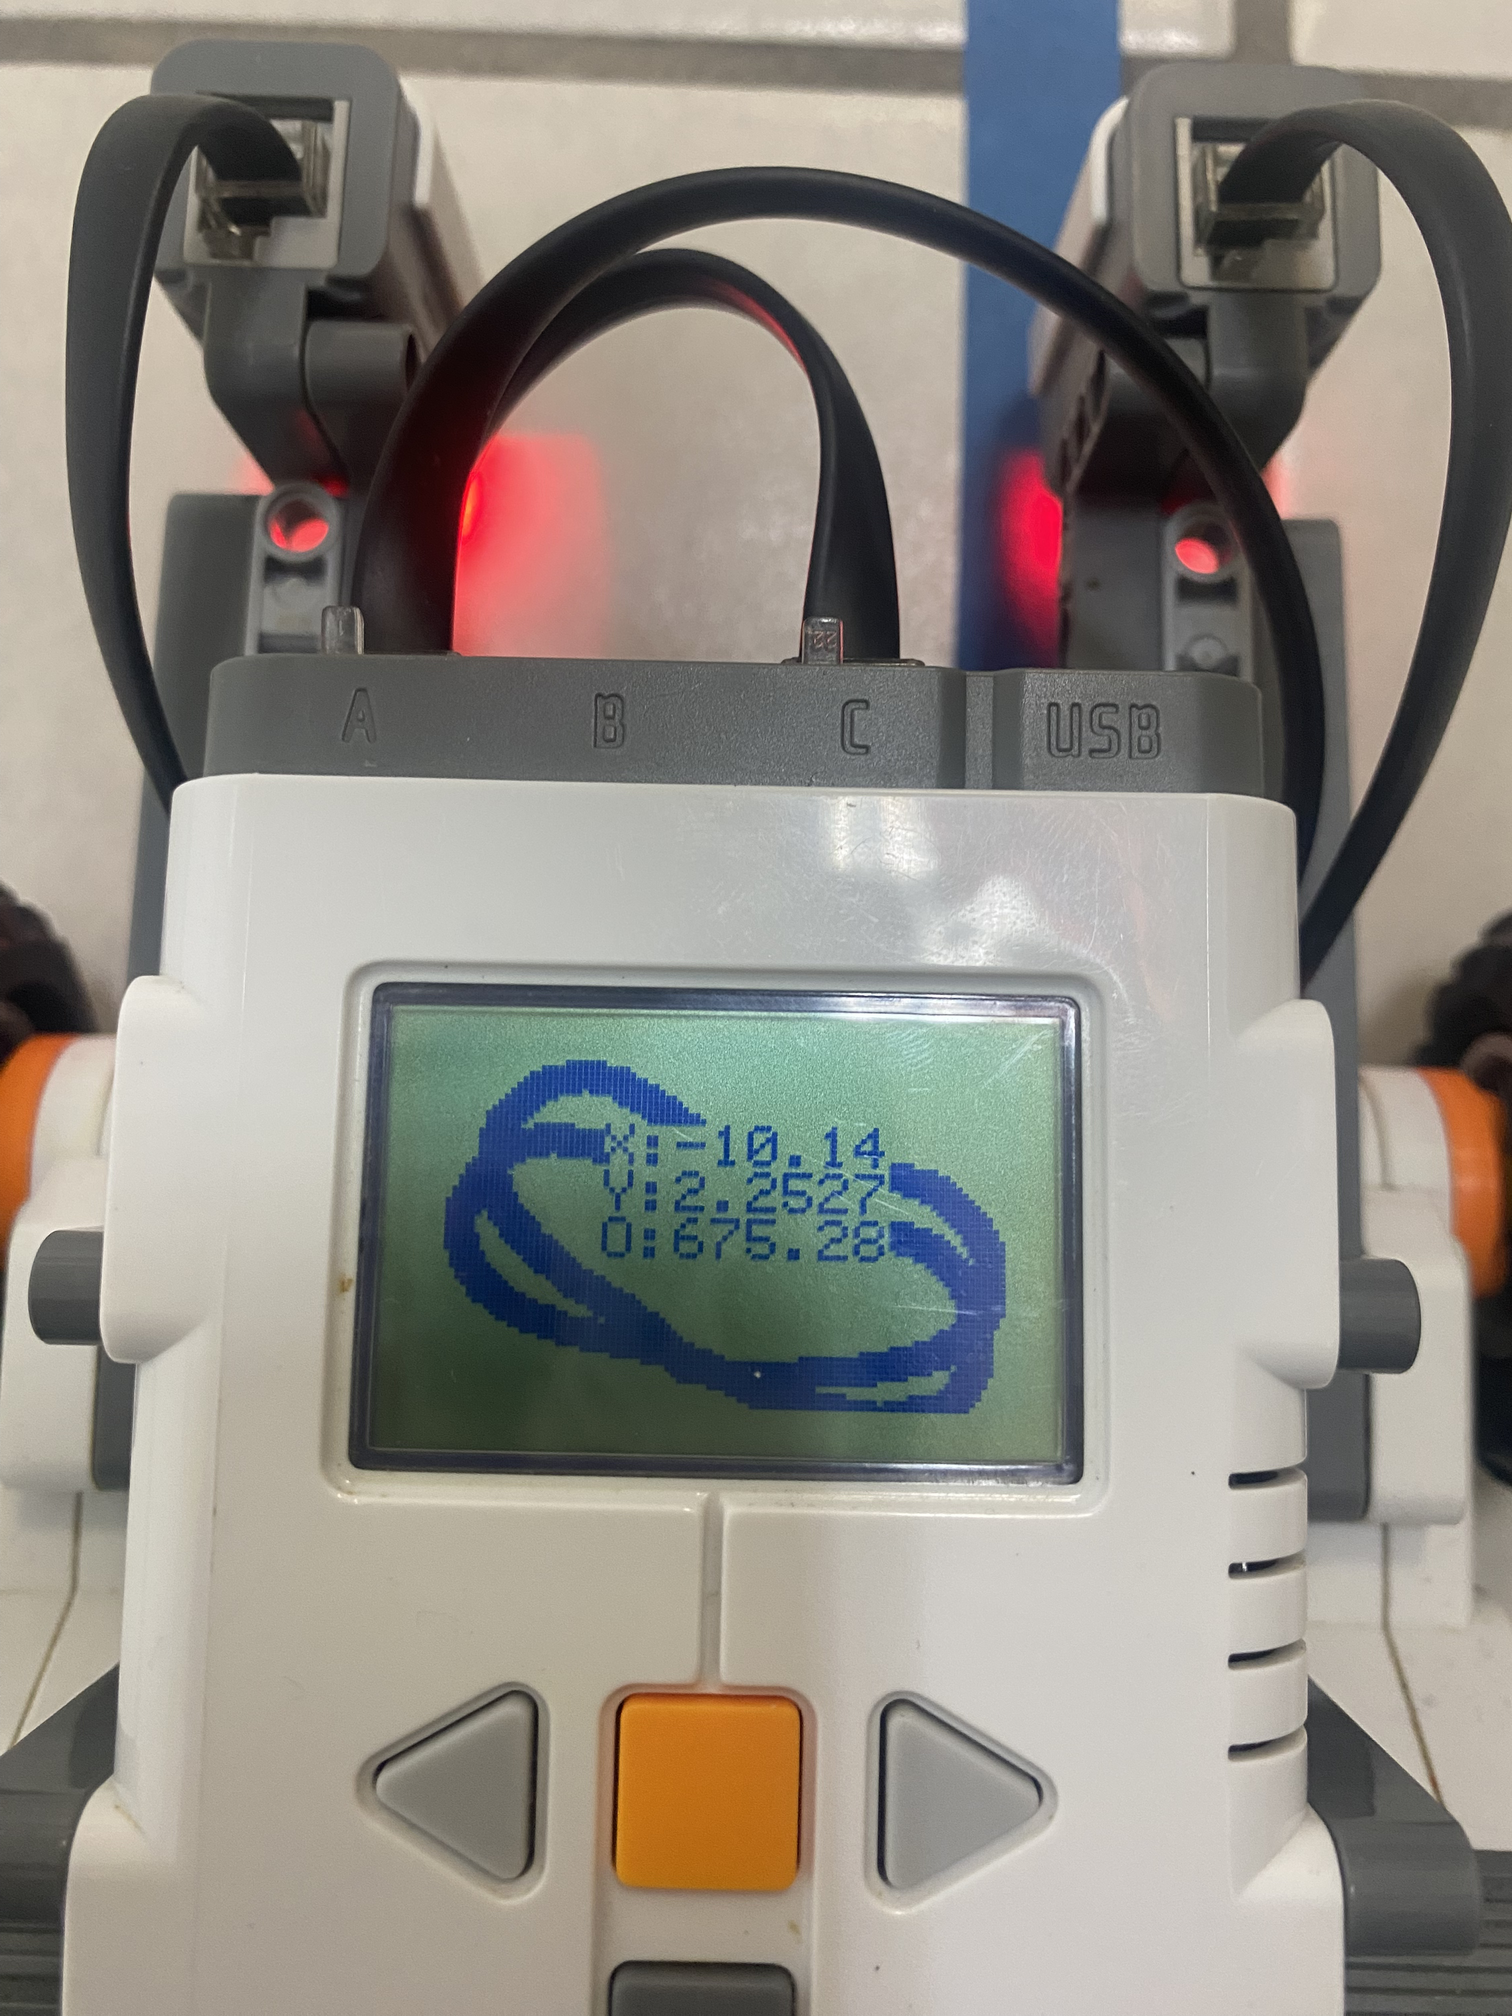
\includegraphics[scale=0.09]{graficos/corrida2.png}
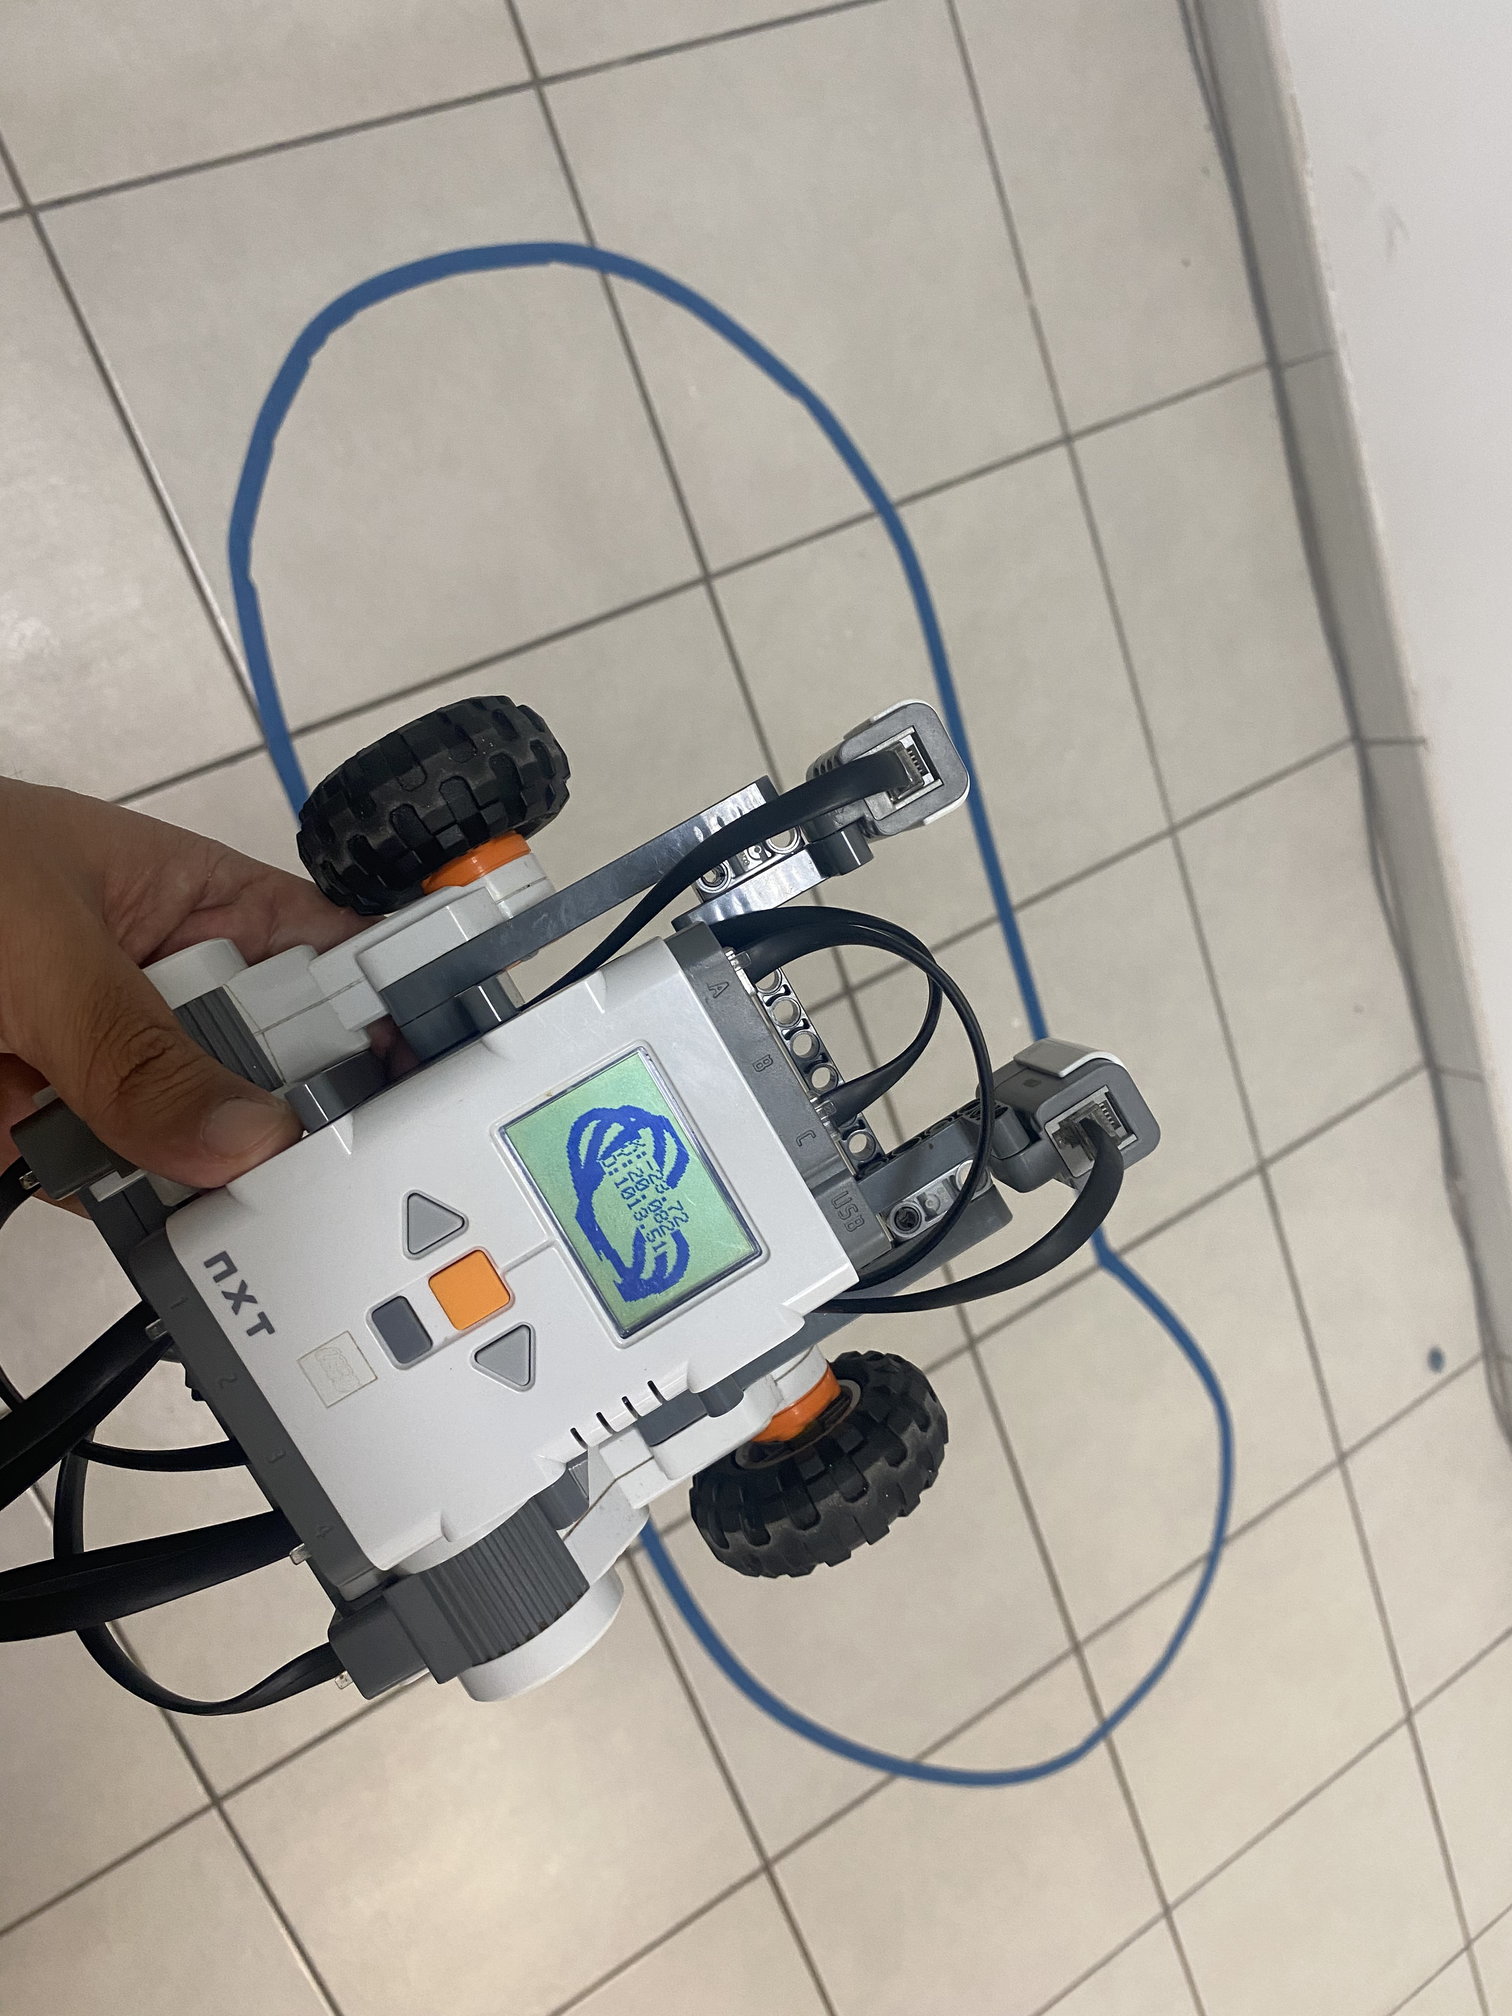
\includegraphics[scale=0.09]{graficos/corrida3.png}
\\\\
Al superponer los recorridos, donde se observa el error por la oscilación originado de la colocación de los sensores que es amplio.

%------------------------------------------------
\newpage
\twocolumn
\section{Resultados}

Los resultados de la estimación de la posición están dentro de lo esperado, teniendo en cuenta la precisión de los sensores y motores. Al cabo de varios metros recorridos el error empieza
a ser considerable. Lo que más error produce son las trayectorias curvas, ya que los rozamientos hacen que los cálculos hechos con las lecturas de los tacómetros de los motores introduzcan demasiado error cuando el robot está girando.\\

%------------------------------------------------
\section{Conclusiones}

En conclusión, la odometría es un método comúnmente utilizado para estimar la posición y orientación de un robot móvil en un entorno desconocido. Sin embargo, como cualquier técnica de medición, la odometría tiene errores que pueden afectar la estimación de la posición y orientación del robot.\\

Los errores sistemáticos en la odometría pueden deberse a una variedad de factores, como el desgaste de las ruedas, la fricción en la superficie del suelo y la falta de precisión en los sensores utilizados para medir la velocidad de las ruedas. Estos errores pueden acumularse con el tiempo y afectar la capacidad del robot para navegar en un ambiente desconocido.\\

Para reducir los errores, es importente realizar una calibración de las mediciones de los encoders y el mantenimiento/ajuste del robot.\\

En resumen, aunque los erres sistemáticos son un desafío importante en la odometría, existen formas de minimizar su impacto y mejorar la precisión de la navegación del robot móvil. Es clave comprender y atender los errores de manera efectiva para lograr un rendimiento óptimo en la navegación autónoma del robot.

%----------------------------------------------------------------------------------------
%	REFERENCE LIST
%----------------------------------------------------------------------------------------

\begin{thebibliography}{0} % Bibliography - this is intentionally simple in this template

  \href{http://ubuntudaily.blogspot.com/2011/03/using-lego-mindstorms-nxt-with-ubuntu.html}{Instalación NXC en Linux}\\\\
  \href{https://github.com/pierre-24/nbc-compiler}{Repositorio NBC utilizado}\\\\
  \href{https://bricxcc.sourceforge.net/nbc/doc/nxtlinux.txt}{Documento para evitar el sudo en el comando NXC}\\\\
  \href{https://howtoinstall.co/en/libusb-dev}{Comando para instalar libusb-dev}\\\\
  \href{http://www.kramirez.net/Robotica/Material/Presentaciones/Odometria.pdf}{Presentación Odometría}\\\\
  \href{https://www.redalyc.org/pdf/849/84916680034.pdf}{VALENCIA V., JHONNY A.; MONTOYA O., ALEJANDRO; RIOS, LUIS HERNANDO
MODELO CINEMÁTICO DE UN ROBOT MÓVIL TIPO DIFERENCIAL Y NAVEGACIÓN A PARTIR DE
LA ESTIMACIÓN ODOMÉTRICA}\\\\
  \href{https://www.google.com/url?sa=t&rct=j&q=&esrc=s&source=web&cd=&cad=rja&uact=8&ved=2ahUKEwiu0_So28_9AhViDkQIHRlXDtcQFnoECBQQAQ&url=https%3A%2F%2Frevistas.udistrital.edu.co%2Findex.php%2FTecnura%2Farticle%2Fdownload%2F6810%2F8394%2F30717&usg=AOvVaw2PsCrkFGkk_nGN-G084B11}{Modelo Cinemático de un robot móvil implementado con LEGO NXT para un sistema de localización indoor diseñado en Labview}
  
  
\end{thebibliography}

%----------------------------------------------------------------------------------------

\end{document}
